% Options for packages loaded elsewhere
\PassOptionsToPackage{unicode}{hyperref}
\PassOptionsToPackage{hyphens}{url}
\PassOptionsToPackage{dvipsnames,svgnames,x11names}{xcolor}
%
\documentclass[
  letterpaper,
  DIV=11,
  numbers=noendperiod]{scrreprt}

\usepackage{amsmath,amssymb}
\usepackage{lmodern}
\usepackage{iftex}
\ifPDFTeX
  \usepackage[T1]{fontenc}
  \usepackage[utf8]{inputenc}
  \usepackage{textcomp} % provide euro and other symbols
\else % if luatex or xetex
  \usepackage{unicode-math}
  \defaultfontfeatures{Scale=MatchLowercase}
  \defaultfontfeatures[\rmfamily]{Ligatures=TeX,Scale=1}
  \setmonofont[]{JuliaMono}
\fi
% Use upquote if available, for straight quotes in verbatim environments
\IfFileExists{upquote.sty}{\usepackage{upquote}}{}
\IfFileExists{microtype.sty}{% use microtype if available
  \usepackage[]{microtype}
  \UseMicrotypeSet[protrusion]{basicmath} % disable protrusion for tt fonts
}{}
\makeatletter
\@ifundefined{KOMAClassName}{% if non-KOMA class
  \IfFileExists{parskip.sty}{%
    \usepackage{parskip}
  }{% else
    \setlength{\parindent}{0pt}
    \setlength{\parskip}{6pt plus 2pt minus 1pt}}
}{% if KOMA class
  \KOMAoptions{parskip=half}}
\makeatother
\usepackage{xcolor}
\usepackage[normalem]{ulem}
\setlength{\emergencystretch}{3em} % prevent overfull lines
\setcounter{secnumdepth}{5}
% Make \paragraph and \subparagraph free-standing
\ifx\paragraph\undefined\else
  \let\oldparagraph\paragraph
  \renewcommand{\paragraph}[1]{\oldparagraph{#1}\mbox{}}
\fi
\ifx\subparagraph\undefined\else
  \let\oldsubparagraph\subparagraph
  \renewcommand{\subparagraph}[1]{\oldsubparagraph{#1}\mbox{}}
\fi

\usepackage{color}
\usepackage{fancyvrb}
\newcommand{\VerbBar}{|}
\newcommand{\VERB}{\Verb[commandchars=\\\{\}]}
\DefineVerbatimEnvironment{Highlighting}{Verbatim}{commandchars=\\\{\}}
% Add ',fontsize=\small' for more characters per line
\usepackage{framed}
\definecolor{shadecolor}{RGB}{241,243,245}
\newenvironment{Shaded}{\begin{snugshade}}{\end{snugshade}}
\newcommand{\AlertTok}[1]{\textcolor[rgb]{0.68,0.00,0.00}{#1}}
\newcommand{\AnnotationTok}[1]{\textcolor[rgb]{0.37,0.37,0.37}{#1}}
\newcommand{\AttributeTok}[1]{\textcolor[rgb]{0.40,0.45,0.13}{#1}}
\newcommand{\BaseNTok}[1]{\textcolor[rgb]{0.68,0.00,0.00}{#1}}
\newcommand{\BuiltInTok}[1]{\textcolor[rgb]{0.00,0.23,0.31}{#1}}
\newcommand{\CharTok}[1]{\textcolor[rgb]{0.13,0.47,0.30}{#1}}
\newcommand{\CommentTok}[1]{\textcolor[rgb]{0.37,0.37,0.37}{#1}}
\newcommand{\CommentVarTok}[1]{\textcolor[rgb]{0.37,0.37,0.37}{\textit{#1}}}
\newcommand{\ConstantTok}[1]{\textcolor[rgb]{0.56,0.35,0.01}{#1}}
\newcommand{\ControlFlowTok}[1]{\textcolor[rgb]{0.00,0.23,0.31}{#1}}
\newcommand{\DataTypeTok}[1]{\textcolor[rgb]{0.68,0.00,0.00}{#1}}
\newcommand{\DecValTok}[1]{\textcolor[rgb]{0.68,0.00,0.00}{#1}}
\newcommand{\DocumentationTok}[1]{\textcolor[rgb]{0.37,0.37,0.37}{\textit{#1}}}
\newcommand{\ErrorTok}[1]{\textcolor[rgb]{0.68,0.00,0.00}{#1}}
\newcommand{\ExtensionTok}[1]{\textcolor[rgb]{0.00,0.23,0.31}{#1}}
\newcommand{\FloatTok}[1]{\textcolor[rgb]{0.68,0.00,0.00}{#1}}
\newcommand{\FunctionTok}[1]{\textcolor[rgb]{0.28,0.35,0.67}{#1}}
\newcommand{\ImportTok}[1]{\textcolor[rgb]{0.00,0.46,0.62}{#1}}
\newcommand{\InformationTok}[1]{\textcolor[rgb]{0.37,0.37,0.37}{#1}}
\newcommand{\KeywordTok}[1]{\textcolor[rgb]{0.00,0.23,0.31}{#1}}
\newcommand{\NormalTok}[1]{\textcolor[rgb]{0.00,0.23,0.31}{#1}}
\newcommand{\OperatorTok}[1]{\textcolor[rgb]{0.37,0.37,0.37}{#1}}
\newcommand{\OtherTok}[1]{\textcolor[rgb]{0.00,0.23,0.31}{#1}}
\newcommand{\PreprocessorTok}[1]{\textcolor[rgb]{0.68,0.00,0.00}{#1}}
\newcommand{\RegionMarkerTok}[1]{\textcolor[rgb]{0.00,0.23,0.31}{#1}}
\newcommand{\SpecialCharTok}[1]{\textcolor[rgb]{0.37,0.37,0.37}{#1}}
\newcommand{\SpecialStringTok}[1]{\textcolor[rgb]{0.13,0.47,0.30}{#1}}
\newcommand{\StringTok}[1]{\textcolor[rgb]{0.13,0.47,0.30}{#1}}
\newcommand{\VariableTok}[1]{\textcolor[rgb]{0.07,0.07,0.07}{#1}}
\newcommand{\VerbatimStringTok}[1]{\textcolor[rgb]{0.13,0.47,0.30}{#1}}
\newcommand{\WarningTok}[1]{\textcolor[rgb]{0.37,0.37,0.37}{\textit{#1}}}

\providecommand{\tightlist}{%
  \setlength{\itemsep}{0pt}\setlength{\parskip}{0pt}}\usepackage{longtable,booktabs,array}
\usepackage{calc} % for calculating minipage widths
% Correct order of tables after \paragraph or \subparagraph
\usepackage{etoolbox}
\makeatletter
\patchcmd\longtable{\par}{\if@noskipsec\mbox{}\fi\par}{}{}
\makeatother
% Allow footnotes in longtable head/foot
\IfFileExists{footnotehyper.sty}{\usepackage{footnotehyper}}{\usepackage{footnote}}
\makesavenoteenv{longtable}
\usepackage{graphicx}
\makeatletter
\def\maxwidth{\ifdim\Gin@nat@width>\linewidth\linewidth\else\Gin@nat@width\fi}
\def\maxheight{\ifdim\Gin@nat@height>\textheight\textheight\else\Gin@nat@height\fi}
\makeatother
% Scale images if necessary, so that they will not overflow the page
% margins by default, and it is still possible to overwrite the defaults
% using explicit options in \includegraphics[width, height, ...]{}
\setkeys{Gin}{width=\maxwidth,height=\maxheight,keepaspectratio}
% Set default figure placement to htbp
\makeatletter
\def\fps@figure{htbp}
\makeatother

\usepackage{mathrsfs}
\usepackage{twemojis}
\usepackage{myunixode}

\makeatletter
\def\squiggly{\bgroup \markoverwith{\textcolor{red}{\lower3.5\p@\hbox{\sixly \char58}}}\ULon}
\makeatother

\renewcommand{\NormalTok}[1]{\textcolor[HTML]{000000}{#1}}
\renewcommand{\KeywordTok}[1]{\textcolor[HTML]{0000FF}{#1}}
\renewcommand{\SpecialCharTok}[1]{}
\renewcommand{\ErrorTok}[1]{\squiggly{#1}}
\renewcommand{\WarningTok}[1]{\squiggly{\textcolor[HTML]{0000FF}{#1}}}
\renewcommand{\StringTok}[1]{\textcolor[HTML]{A52A2A}{#1}}
\renewcommand{\CommentTok}[1]{\textcolor[HTML]{008000}{#1}}
\renewcommand{\InformationTok}[1]{\textcolor[HTML]{D2691E}{\textbf{#1}}}

%redefines Shaded so it can't break
\newcommand{\nobreakShaded}{\renewenvironment{Shaded}
	{\begin{tcolorbox}[frame hidden, enhanced, interior hidden, boxrule=0pt,
		borderline west={3pt}{0pt}{shadecolor}, sharp corners]}
	{\end{tcolorbox}}}

%Make end of environment ignore pars that come after it
\def\useignorespacesandallpars#1\ignorespaces\fi{%
#1\fi\ignorespacesandallpars}

\makeatletter
\def\ignorespacesandallpars{%
  \@ifnextchar\par
    {\expandafter\ignorespacesandallpars\@gobble}%
    {}%
}
\makeatother

\newenvironment{inpt}
	{\nobreakShaded\noindent\begin{minipage}[t]{0.63\textwidth}}
	{\end{minipage}\hfill\useignorespacesandallpars}

\newenvironment{outpt}
	{\nobreakShaded\begin{minipage}[t]{0.32\textwidth}}
	{\end{minipage}}

\newenvironment{lft}
	{\nobreakShaded\noindent\begin{minipage}[t]{0.475\textwidth}}
	{\end{minipage}\hfill\useignorespacesandallpars}

\newenvironment{rt}
	{\nobreakShaded\begin{minipage}[t]{0.475\textwidth}}
	{\end{minipage}}

\newcommand{\excl}[1]{}
\newcommand{\incl}[1]{#1}
\KOMAoption{captions}{tableheading}
\makeatletter
\makeatother
\makeatletter
\@ifpackageloaded{bookmark}{}{\usepackage{bookmark}}
\makeatother
\makeatletter
\@ifpackageloaded{caption}{}{\usepackage{caption}}
\AtBeginDocument{%
\ifdefined\contentsname
  \renewcommand*\contentsname{Table of contents}
\else
  \newcommand\contentsname{Table of contents}
\fi
\ifdefined\listfigurename
  \renewcommand*\listfigurename{List of Figures}
\else
  \newcommand\listfigurename{List of Figures}
\fi
\ifdefined\listtablename
  \renewcommand*\listtablename{List of Tables}
\else
  \newcommand\listtablename{List of Tables}
\fi
\ifdefined\figurename
  \renewcommand*\figurename{Figure}
\else
  \newcommand\figurename{Figure}
\fi
\ifdefined\tablename
  \renewcommand*\tablename{Table}
\else
  \newcommand\tablename{Table}
\fi
}
\@ifpackageloaded{float}{}{\usepackage{float}}
\floatstyle{ruled}
\@ifundefined{c@chapter}{\newfloat{codelisting}{h}{lop}}{\newfloat{codelisting}{h}{lop}[chapter]}
\floatname{codelisting}{Listing}
\newcommand*\listoflistings{\listof{codelisting}{List of Listings}}
\makeatother
\makeatletter
\@ifpackageloaded{caption}{}{\usepackage{caption}}
\@ifpackageloaded{subcaption}{}{\usepackage{subcaption}}
\makeatother
\makeatletter
\@ifpackageloaded{tcolorbox}{}{\usepackage[many]{tcolorbox}}
\makeatother
\makeatletter
\@ifundefined{shadecolor}{\definecolor{shadecolor}{rgb}{.97, .97, .97}}
\makeatother
\makeatletter
\makeatother
\ifLuaTeX
  \usepackage{selnolig}  % disable illegal ligatures
\fi
\IfFileExists{bookmark.sty}{\usepackage{bookmark}}{\usepackage{hyperref}}
\IfFileExists{xurl.sty}{\usepackage{xurl}}{} % add URL line breaks if available
\urlstyle{same} % disable monospaced font for URLs
\hypersetup{
  pdftitle={How To Prove It With Lean},
  pdfauthor={Daniel J. Velleman},
  colorlinks=true,
  linkcolor={blue},
  filecolor={Maroon},
  citecolor={Blue},
  urlcolor={Blue},
  pdfcreator={LaTeX via pandoc}}

\title{How To Prove It With Lean}
\author{Daniel J. Velleman}
\date{}

\begin{document}
\maketitle
\ifdefined\Shaded\renewenvironment{Shaded}{\begin{tcolorbox}[breakable, interior hidden, borderline west={3pt}{0pt}{shadecolor}, boxrule=0pt, enhanced, sharp corners, frame hidden]}{\end{tcolorbox}}\fi

\renewcommand*\contentsname{Table of contents}
{
\hypersetup{linkcolor=}
\setcounter{tocdepth}{1}
\tableofcontents
}
\bookmarksetup{startatroot}

\hypertarget{preface}{%
\chapter*{Preface}\label{preface}}
\addcontentsline{toc}{chapter}{Preface}

\hypertarget{about-this-book}{%
\section*{About This Book}\label{about-this-book}}
\addcontentsline{toc}{section}{About This Book}

This book is intended to accompany my book
\href{https://www.cambridge.org/highereducation/books/how-to-prove-it/6D2965D625C6836CD4A785A2C843B3DA\#overview}{\emph{How
To Prove It}} (henceforth called \emph{HTPI}), which is published by
Cambridge University Press. Although this book is self-contained, we
will sometimes have occasion to refer to passages in \emph{HTPI}, so
this book will be easiest to understand if you have a copy of
\emph{HTPI} available to you.

\emph{HTPI} explains a systematic approach to constructing mathematical
proofs. The purpose of this book is to show you how to use a computer
software package called \emph{Lean} to help you master the techniques
presented in \emph{HTPI}. Lean is free software that is available for
Windows, MacOS, and Unix computers. To get the most out of this book,
you will need to download and install Lean on your computer. We will
explain how to do that below.

The chapters and sections of this book are numbered to match the
sections of \emph{HTPI} to which they correspond. The first two chapters
of \emph{HTPI} cover preliminary topics in elementary logic and set
theory that are needed to understand the proof techniques presented in
later chapters. We assume that you are already familiar with that
material (if not, go read those chapters in \emph{HTPI} !), so Chapters
1 and 2 of this book will just briefly summarize the most important
points. Those chapters are followed by an introduction to Lean that
explains the basics of using Lean to write proofs. The presentation of
proof techniques in \emph{HTPI} begins in earnest in Chapter 3, so that
is where we will begin to discuss how Lean can be used to master those
techniques.

If you are reading this book online, then you will find a search box in
the left margin. You can use that box to search for any word or phrase
anywhere in the book. Below the search box is a list of the chapters of
the book. Click on any chapter to go to that chapter. Within each
chapter, a table of contents in the right margin lists the sections in
that chapter. Again, you can go to any section by clicking on it. At the
end of each chapter there are links to take you to the next or previous
chapter.

\hypertarget{about-lean}{%
\section*{About Lean}\label{about-lean}}
\addcontentsline{toc}{section}{About Lean}

Lean is a kind of software package called a \emph{proof assistant}. What
that means is that Lean can help you to write proofs. As we will see
over the course of this book, there are several ways in which Lean can
be helpful. First of all, if you type a proof into Lean, then Lean can
check the correctness of the proof and point out errors. As you are
typing a proof into Lean, it will keep track of what has been
accomplished so far in the proof and what remains to be done to finish
the proof, and it will display that information for you. That can keep
you moving in the right direction as you are figuring out a proof. And
sometimes Lean can fill in small details of the proof for you.

Of course, to make this possible you must type your proof in a format
that Lean understands. Much of this book will be taken up with
explaining how to write a proof so that Lean will understand it.

\hypertarget{installing-lean}{%
\section*{Installing Lean}\label{installing-lean}}
\addcontentsline{toc}{section}{Installing Lean}

We will be using Visual Studio Code to run Lean, so you will need to
install VS Code first. VS Code is free and can be downloaded
\href{https://code.visualstudio.com}{here}.

You will also need the Lean package that accompanies this book, which
can be downloaded from
\url{https://github.com/djvelleman/HTPILeanPackage}. After following the
link, click on the green ``Code'' button and, in the pop-up menu, select
``Download ZIP''. Open the downloaded zip file to create a folder
containing the HTPI Lean package. You can put this folder wherever you
want on your computer.

Now open VS Code. You should see a window that looks something like
this:


\includegraphics{./Images/VSCodeStart.png}

Click on the \emph{Extensions} icon on the left side of the window,
which is circled in red in the image above. That will bring up a list of
available extensions:


\includegraphics{./Images/FindExtension.png}

In the \emph{Search Extensions in Marketplace} field, type ``lean4''. VS
Code should find the Lean 4 extension and display it:


\includegraphics{./Images/InstallExtension.png}

Click on ``Install'' to install the Lean 4 extension.

Next, in VS Code, select ``Open Folder \ldots{}'' from the File menu and
open the folder containing the HTPI Lean package that you downloaded
earlier. Under the heading ``Explorer'' on the left side of the window,
you should see a list of the files in the package. (If you don't see the
list, try clicking on the \emph{Explorer} icon, circled in red below.)

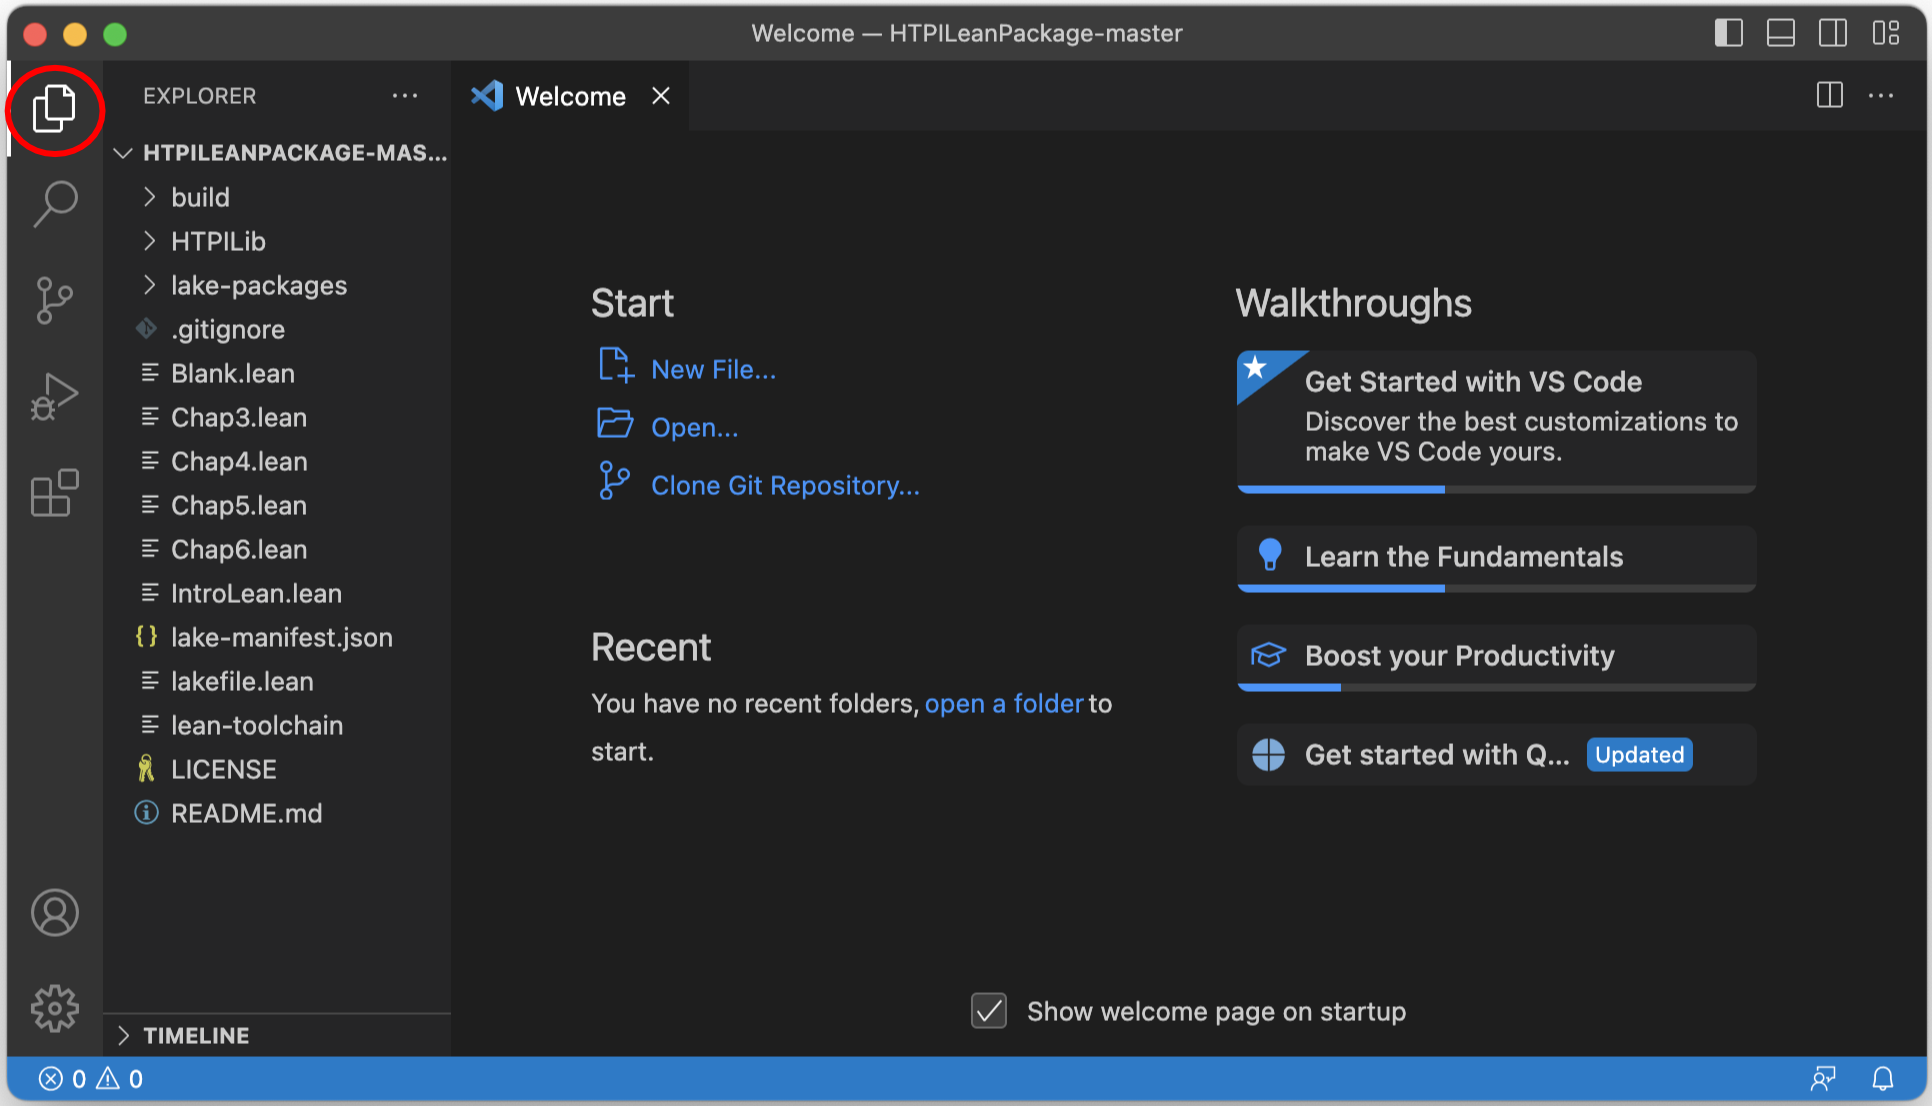
\includegraphics{./Images/OpenPackage.png}

Click on the file ``Blank.lean'' in the file list. You should see a
warning that VS Code failed to start the `lean' language server:

\begin{figure}

{\centering 
\includegraphics{./Images/Install-elan.png}

}

\end{figure}

Click on the ``Install Lean using Elan'' button, and the Lean server
should be installed. This may take a while, and there may be messages
asking you to do things. If anything goes wrong, try quiting VS Code and
restarting. Eventually your window should look like this:

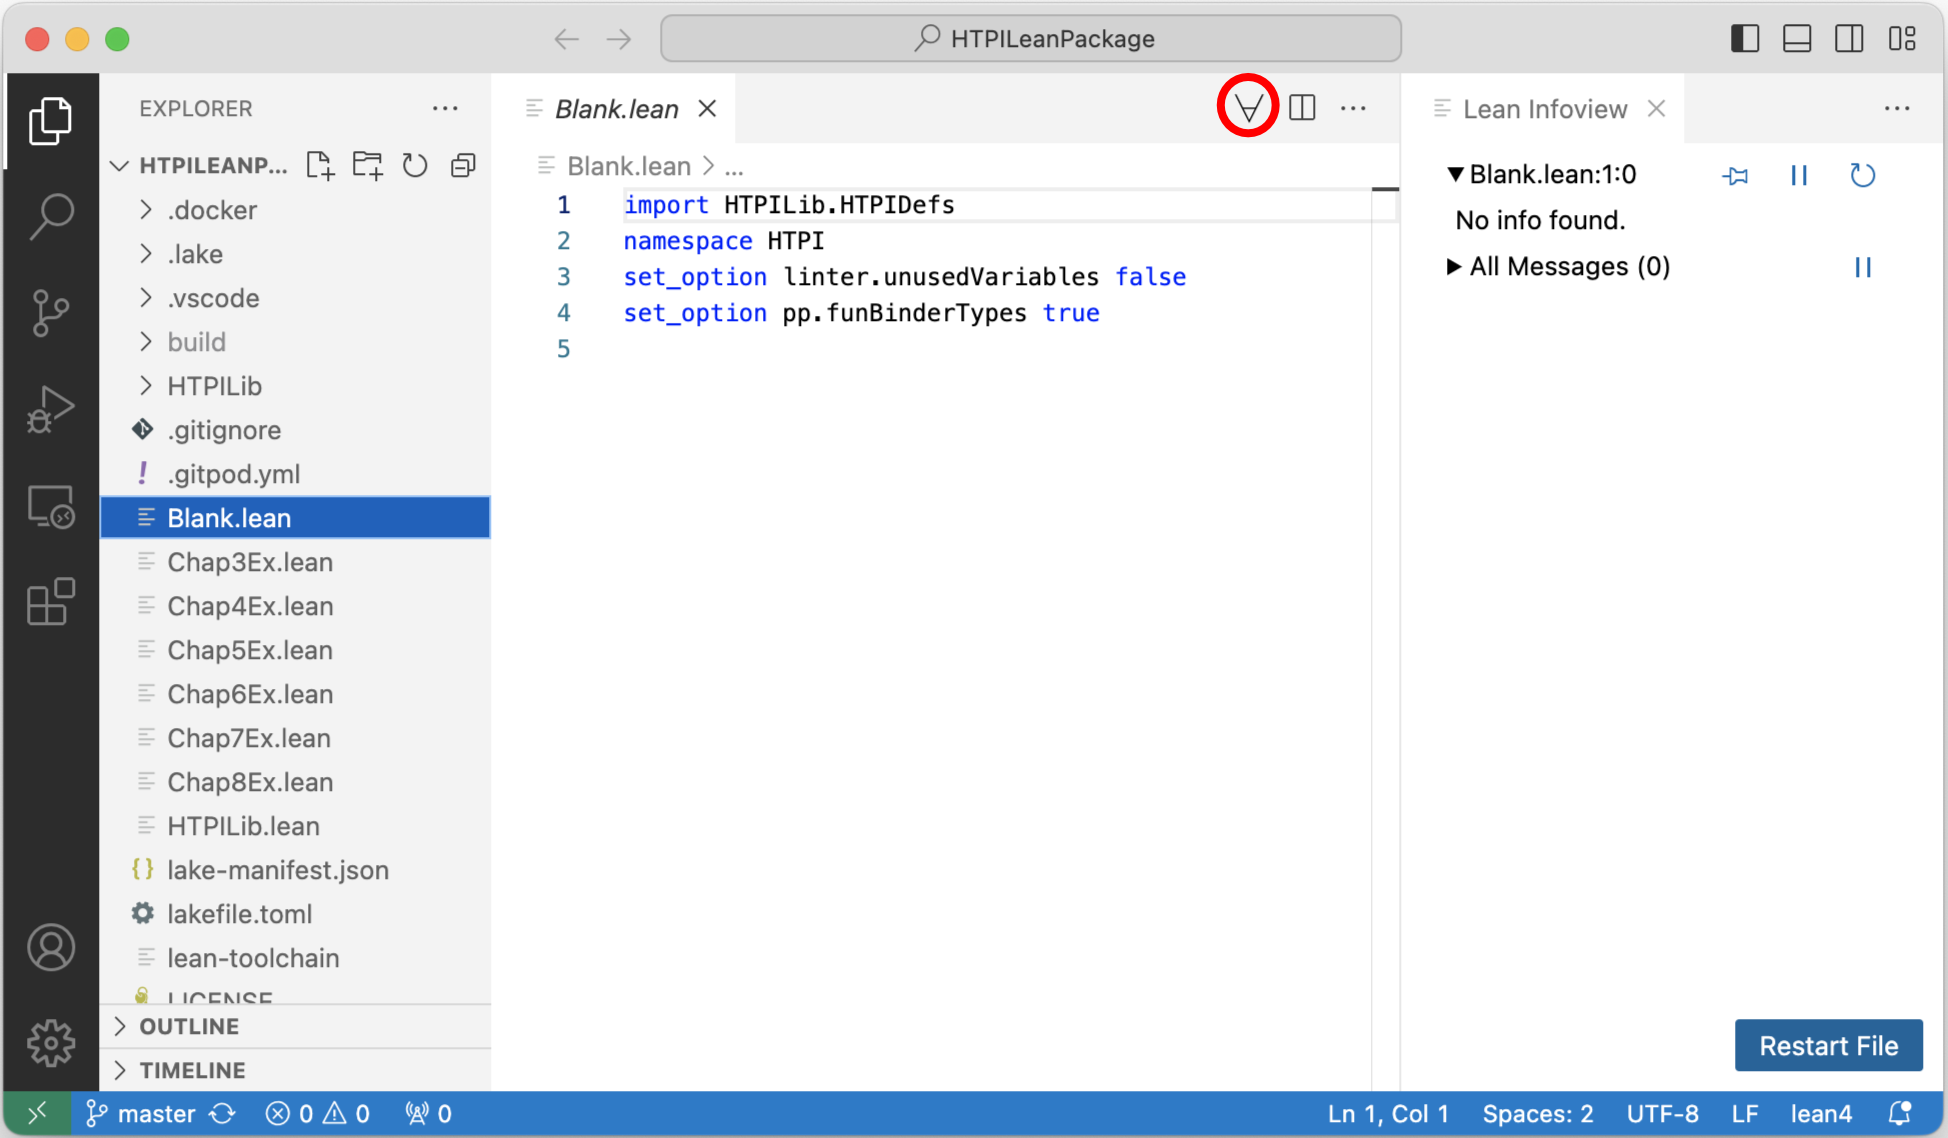
\includegraphics{./Images/Ready.png}

If you don't see the Infoview pane on the right side of the window,
click on the icon circled in red in the image above, and the Infoview
pane should appear.

Your installation is now complete.

\bookmarksetup{startatroot}

\hypertarget{sentential-logic}{%
\chapter{Sentential Logic}\label{sentential-logic}}

Chapter 1 of \emph{How To Prove It} introduces the following symbols of
logic:

\begin{longtable}[]{@{}cc@{}}
\toprule()
Symbol & Meaning \\
\midrule()
\endhead
\(\neg\) & not \\
\(\wedge\) & and \\
\(\vee\) & or \\
\(\to\) & if \ldots{} then \\
\(\leftrightarrow\) & if and only if \\
\bottomrule()
\end{longtable}

As we will see, Lean uses the same symbols, with the same meanings. This
chapter also establishes a number of logical equivalences that will be
useful to us later:

\hypertarget{prop-laws}{}
\begin{longtable}[]{@{}
  >{\raggedright\arraybackslash}p{(\columnwidth - 6\tabcolsep) * \real{0.3226}}
  >{\centering\arraybackslash}p{(\columnwidth - 6\tabcolsep) * \real{0.2258}}
  >{\centering\arraybackslash}p{(\columnwidth - 6\tabcolsep) * \real{0.2258}}
  >{\centering\arraybackslash}p{(\columnwidth - 6\tabcolsep) * \real{0.2258}}@{}}
\toprule()
\begin{minipage}[b]{\linewidth}\raggedright
Name
\end{minipage} & \begin{minipage}[b]{\linewidth}\centering
\end{minipage} & \begin{minipage}[b]{\linewidth}\centering
Equivalence
\end{minipage} & \begin{minipage}[b]{\linewidth}\centering
\end{minipage} \\
\midrule()
\endhead
De Morgan's Laws & \(\neg (P \wedge Q)\) & is equivalent to &
\(\neg P \vee \neg Q\) \\
& \(\neg (P \vee Q)\) & is equivalent to & \(\neg P \wedge \neg Q\) \\
Double Negation Law & \(\neg\neg P\) & is equivalent to & \(P\) \\
Conditional Laws & \(P \to Q\) & is equivalent to & \(\neg P \vee Q\) \\
& \(P \to Q\) & is equivalent to & \(\neg(P \wedge \neg Q)\) \\
Contrapositive Law & \(P \to Q\) & is equivalent to &
\(\neg Q \to \neg P\) \\
\bottomrule()
\end{longtable}

Finally, Chapter 1 of \emph{HTPI} introduces some concepts from set
theory. A \emph{set} is a collection of objects; the objects in the
collection are called \emph{elements} of the set. If \(P(x)\) is a
statement about \(x\), then \(\{x \mid P(x)\}\) denotes the set whose
elements are the objects \(x\) for which \(P(x)\) is true. The notation
\(x \in A\) means that \(x\) is an element of \(A\). Two sets \(A\) and
\(B\) are \emph{equal} if they have exactly the same elements. We say
that \(A\) is a \emph{subset} of \(B\), denoted \(A \subseteq B\), if
every element of \(A\) is an element of \(B\). And we have the following
operations on sets:

\begin{quote}
\(A \cap B = \{x \mid x \in A \wedge x \in B\} = {}\) the
\emph{intersection} of \(A\) and \(B\),

\(A \cup B = \{x \mid x \in A \vee x \in B\} = {}\) the \emph{union} of
\(A\) and \(B\),

\(A \mathbin{\backslash} B = \{x \mid x \in A \wedge x \notin B\} = {}\)
the \emph{difference} of \(A\) and \(B\),

\(A \bigtriangleup B = (A \mathbin{\backslash} B) \cup (B \mathbin{\backslash} A) = {}\)
the \emph{symmetric difference} of \(A\) and \(B\).

\end{quote}

\bookmarksetup{startatroot}

\hypertarget{quantificational-logic}{%
\chapter{Quantificational Logic}\label{quantificational-logic}}

Chapter 2 of \emph{How To Prove It} introduces two more symbols of
logic, the quantifiers \(\forall\) and \(\exists\). If \(P(x)\) is a
statement about an object \(x\), then

\begin{quote}
\(\forall x\,P(x)\) means ``for all \(x\), \(P(x)\),''

\end{quote}

and

\begin{quote}
\(\exists x\,P(x)\) means ``there exists some \(x\) such that
\(P(x)\).''

\end{quote}

Lean also uses these symbols, although we will see that quantified
statements are written slightly differently in Lean from the way they
are written in \emph{HTPI}. In the statement \(P(x)\), the variable
\(x\) is called a \emph{free variable}. But in \(\forall x\,P(x)\) or
\(\exists x\,P(x)\), it is a \emph{bound variable}; we say that the
quantifiers \(\forall\) and \(\exists\) \emph{bind} the variable.

Once again, there are logical equivalences involving these symbols that
will be useful to us later:

\begin{longtable}[]{@{}
  >{\raggedright\arraybackslash}p{(\columnwidth - 6\tabcolsep) * \real{0.3226}}
  >{\centering\arraybackslash}p{(\columnwidth - 6\tabcolsep) * \real{0.2258}}
  >{\centering\arraybackslash}p{(\columnwidth - 6\tabcolsep) * \real{0.2258}}
  >{\centering\arraybackslash}p{(\columnwidth - 6\tabcolsep) * \real{0.2258}}@{}}
\toprule()
\begin{minipage}[b]{\linewidth}\raggedright
Name
\end{minipage} & \begin{minipage}[b]{\linewidth}\centering
\end{minipage} & \begin{minipage}[b]{\linewidth}\centering
Equivalence
\end{minipage} & \begin{minipage}[b]{\linewidth}\centering
\end{minipage} \\
\midrule()
\endhead
Quantifier Negation Laws & \(\neg \exists x\,P(x)\) & is equivalent to &
\(\forall x\,\neg P(x)\) \\
& \(\neg \forall x\,P(x)\) & is equivalent to &
\(\exists x\,\neg P(x)\) \\
\bottomrule()
\end{longtable}

Chapter 2 of \emph{HTPI} also introduces some more advanced set theory
operations. For any set \(A\),

\begin{quote}
\(\mathscr{P}(A) = \{X \mid X \subseteq A\} = {}\) the \emph{power set}
of \(A\).

\end{quote}

Also, if \(\mathcal{F}\) is a family of sets---that is, a set whose
elements are sets---then

\begin{quote}
\(\bigcap \mathcal{F} = \{x \mid \forall A(A \in \mathcal{F} \to x \in A)\} = {}\)
the \emph{intersection} of the family \(\mathcal{F}\),

\(\bigcup \mathcal{F} = \{x \mid \exists A(A \in \mathcal{F} \wedge x \in A)\} = {}\)
the \emph{union} of the family \(\mathcal{F}\).

\end{quote}

Finally, Chapter 2 introduces the notation \(\exists ! x\,P(x)\) to mean
``there is exactly one \(x\) such that \(P(x).\)'' This can be thought
of as an abbreviation for
\(\exists x(P(x) \wedge \neg\exists y(P(y) \wedge y \ne x))\). By the
quantifier negation, De Morgan, and conditional laws, this is equivalent
to \(\exists x(P(x) \wedge \forall y(P(y) \to y = x))\).

\bookmarksetup{startatroot}

\hypertarget{introduction-to-lean}{%
\chapter*{Introduction to Lean}\label{introduction-to-lean}}
\addcontentsline{toc}{chapter}{Introduction to Lean}

If you are reading this book in conjunction with \emph{How To Prove It},
you should complete Section 3.2 of \emph{HTPI} before reading this
chapter. Once you have reached that point in \emph{HTPI}, you are ready
to start learning about Lean. In this chapter we'll explain the basics
of writing proofs in Lean and getting feedback from Lean.

\hypertarget{a-first-example}{%
\section*{A First Example}\label{a-first-example}}
\addcontentsline{toc}{section}{A First Example}

We'll start with Example 3.2.4 in \emph{How To Prove It}. Here is how
the theorem and proof in that example appear in \emph{HTPI} (consult
\emph{HTPI} if you want to see how this proof was constructed):

\textbf{Theorem}. \emph{Suppose \(P \to (Q \to R)\). Then
\(\neg R \to (P \to \neg Q)\)}.

Proof. Suppose \(\neg R\). Suppose \(P\). Since \(P\) and
\(P \to (Q \to R)\), it follows that \(Q \to R\). But then, since
\(\neg R\), we can conclude \(\neg Q\). Thus, \(P \to \neg Q\).
Therefore \(\neg R \to (P \to \neg Q)\).

And here is how we would write the proof in Lean:

\begin{Shaded}
\begin{Highlighting}[]
\KeywordTok{theorem}\NormalTok{ Example\_3\_2\_4}
\NormalTok{(P Q R : }\KeywordTok{Prop}\NormalTok{) (h : P → (Q → R)) : ¬R → (P → ¬Q) := }\KeywordTok{by}
  \KeywordTok{assume}\NormalTok{ h2 : ¬R}
  \KeywordTok{assume}\NormalTok{ h3 : P}
  \KeywordTok{have}\NormalTok{ h4 : Q → R := h h3}
  \KeywordTok{contrapos} \KeywordTok{at}\NormalTok{ h4            }\CommentTok{{-}{-}Now h4 : ¬R → ¬Q}
  \KeywordTok{show}\NormalTok{ ¬Q }\KeywordTok{from}\NormalTok{ h4 h2}
\end{Highlighting}
\end{Shaded}

Let's go through this Lean proof line-by-line and see what it means. The
first line tells Lean that we are going to prove a theorem, and it gives
the theorem a name, \texttt{Example\_3\_2\_4}. The next line states the
theorem. In the theorem as stated in \emph{HTPI}, the letters \(P\),
\(Q\), and \(R\) are used to stand for statements that are either true
or false. In logic, such statements are often called
\emph{propositions}. The expression \texttt{(P\ Q\ R\ :\ Prop)} on the
second line tells Lean that \texttt{P}, \texttt{Q}, and \texttt{R} will
be used in this theorem to stand for propositions. The next
parenthetical expression, \texttt{(h\ :\ P\ →\ (Q\ →\ R))}, states the
hypothesis of the theorem and gives it the name \texttt{h}; the
technical term that Lean uses is that \texttt{h} is an \emph{identifier}
for the hypothesis. Assigning an identifier to the hypothesis gives us a
way to refer to it when it is used later in the proof. Almost any string
of characters that doesn't begin with a digit can be used as an
identifier, but it is traditional to use identifiers beginning with the
letter \texttt{h} for hypotheses. After the statement of the hypothesis
there is a colon followed by the conclusion of the theorem,
\texttt{¬R\ →\ (P\ →\ ¬Q)}. Finally, at the end of the second line, the
expression \texttt{:=\ by} signals the beginning of the proof.

Each of the remaining lines is a step in the proof. The first line of
the proof introduces the assumption \texttt{¬R} and gives it the
identifier \texttt{h2}. Of course, this corresponds precisely to the
first sentence of the proof in \emph{HTPI}. Similarly, the second line,
corresponding to the second sentence of the \emph{HTPI} proof, assigns
the identifier \texttt{h3} to the assumption \texttt{P}. The next line
makes the inference \texttt{Q\ →\ R}, giving it the identifier
\texttt{h4}. The inference is justified by combining statements
\texttt{h} and \texttt{h3}---that is, the statements
\texttt{P\ →\ (Q\ →\ R)} and \texttt{P}---exactly as in the third
sentence of the proof in \emph{HTPI}.

The next step of the proof in \emph{HTPI} combines the statements
\(Q \to R\) and \(\neg R\) to draw the inference \(\neg Q\). This
reasoning is justified by the contrapositive law, which says that
\(Q \to R\) is equivalent to its contrapositive, \(\neg R \to \neg Q\).
In the Lean proof, this inference is broken up into two steps. In the
fourth line of the proof, we ask Lean to rewrite statement
\texttt{h4}---that is, \texttt{Q\ →\ R}---using the contrapositive law.
Two hyphens in a row tell Lean that the rest of the line is a comment.
Lean ignores comments and displays them in green. The comment on line
four serves as a reminder that \texttt{h4} now stands for the statement
\texttt{¬R\ →\ ¬Q}. Finally, in the last line of the proof, we combine
the new \texttt{h4} with \texttt{h2} to infer \texttt{¬Q}. There is no
need to give this statement an identifier, because it completes the
proof. In the proof in \emph{HTPI}, there are a couple of final
sentences explaining \emph{why} this completes the proof, but Lean
doesn't require this explanation.

\hypertarget{term-mode}{%
\section*{Term Mode}\label{term-mode}}
\addcontentsline{toc}{section}{Term Mode}

Now that you have seen an example of a proof in Lean, it is time for you
to write your first proof. Lean has two modes for writing proofs, called
\emph{term mode} and \emph{tactic mode}. The example above was written
in tactic mode, and that is the mode we will use for most proofs in this
book. But before we study the construction of proofs in tactic mode, it
will be helpful to learn a bit about term mode. Term mode is best for
simple proofs, so we begin with a few very short proofs.

If you have not yet installed Lean on your computer, go back and follow
the \protect\hyperlink{installing-lean}{instructions} for installing it
now. Then in VS Code, open the folder for the HTPI Lean Package that you
downloaded and click on the file Blank.lean. The file starts with the
line \texttt{import\ HTPIDefs}. Click on the blank line at the end of
the file; this is where you will be typing your first proofs.

Now type in the following theorem and proof:

\begin{Shaded}
\begin{Highlighting}[]
\KeywordTok{theorem}\NormalTok{ extremely\_easy (P : }\KeywordTok{Prop}\NormalTok{) (h : P) : P := h}
\end{Highlighting}
\end{Shaded}

This theorem and proof are so short we have put everything on one line.
In this theorem, the letter \texttt{P} is used to stand for a
proposition. The theorem has one hypothesis, \texttt{P}, which has been
given the identifier \texttt{h}, and the conclusion of the theorem is
also \texttt{P}. The notation \texttt{:=} indicates that what follows
will be a proof in term mode.

Of course, the proof of the theorem is extremely easy: to prove
\texttt{P}, we just have to point out that it is given as the hypothesis
\texttt{h}. And so the proof in Lean consists of just one letter:
\texttt{h}.

Even though this example is a triviality, there are some things to be
learned from it. First of all, although we have been describing the
letter \texttt{h} as an \emph{identifier} for the hypothesis \texttt{P},
this example illustrates that Lean also considers \texttt{h} to be a
\emph{proof} of \texttt{P}. In general, when we see \texttt{h\ :\ P} in
a Lean proof, where \texttt{P} is a proposition, we can think of it as
meaning, not just that \texttt{h} is an identifier for the statement
\texttt{P}, but also that \texttt{h} is a proof of \texttt{P}.

We can learn something else from this example by changing it slightly.
If you change the final \texttt{h} to a different letter---say,
\texttt{f}---you will see that Lean puts a red squiggly line under the
\texttt{f}, like this:

\begin{Shaded}
\begin{Highlighting}[]
\KeywordTok{theorem}\NormalTok{ extremely\_easy (P : }\KeywordTok{Prop}\NormalTok{) (h : P) : P := }\SpecialCharTok{!!}\ErrorTok{f}\SpecialCharTok{!!}
\end{Highlighting}
\end{Shaded}

This indicates that Lean has detected an error in the proof. Lean always
indicates errors by putting a red squiggle under the offending text.
Lean also puts a message in the Lean Infoview pane explaining what the
error is. (If you don't see the Infoview pane, choose ``Command Palette
\ldots{}'' in the ``View'' menu, and then type ``Lean'' in the text box
that appears. You will see a list of commands that start with ``Lean''.
Click on ``Lean 4: Infoview: Toggle'' to make the Infoview pane appear.)
In this case, the message is
\texttt{unknown\ identifier\ \textquotesingle{}f\textquotesingle{}}. The
message is introduced by a heading, in red, that identifies the file,
the line number, and the character position on that line where the error
appears. If you change \texttt{f} back to \texttt{h}, the red squiggle
and error message go away.

Let's try a slightly less trivial example. To type the \texttt{→} symbol
in the next example, type \texttt{\textbackslash{}to} and then hit
either the space bar or the tab key; when you type either space or tab,
the \texttt{\textbackslash{}to} will change to \texttt{→}.
Alternatively, you can type \texttt{\textbackslash{}r} (short for
``right arrow'') or \texttt{\textbackslash{}imp} (short for
``implies''), again followed by either space or tab. Or, you can type
\excl{\texttt{-\textgreater{}}}\texttt{-\null>}, and Lean will interpret
it as \texttt{→}.

\begin{Shaded}
\begin{Highlighting}[]
\KeywordTok{theorem}\NormalTok{ very\_easy}
\NormalTok{(P Q : }\KeywordTok{Prop}\NormalTok{) (h1 : P → Q) (h2 : P) : Q := h1 h2}
\end{Highlighting}
\end{Shaded}

This time there are two hypotheses, \texttt{h1\ :\ P\ →\ Q} and
\texttt{h2\ :\ P}. As explained in Section 3.2 of \emph{HTPI}, the
conclusion \texttt{Q} follows from these hypotheses by the logical rule
\emph{modus ponens}. To use modus ponens to complete this proof in term
mode, we simply write the identifiers of the two hypotheses---which, as
we have just seen, can also be thought of as proofs of the two
hypotheses---one after the other, with a space between them. It is
important to write the proof of the conditional hypothesis first, so the
proof is written \texttt{h1\ h2}; if you try writing this proof as
\texttt{h2\ h1}, you will get a red squiggle. In general, if \texttt{a}
is a proof of any conditional statement \texttt{X\ →\ Y}, and \texttt{b}
is a proof of the antecedent \texttt{X}, then \texttt{a\ b} is a proof
of the consequent \texttt{Y}. The proofs \texttt{a} and \texttt{b} need
not be simply identifiers; any proofs of a conditional statement and its
antecedent can be combined in this way.

We'll try one more proof in term mode:

\begin{Shaded}
\begin{Highlighting}[]
\KeywordTok{theorem}\NormalTok{ easy (P Q R : }\KeywordTok{Prop}\NormalTok{) (h1 : P → Q)}
\NormalTok{(h2 : Q → R) (h3 : P) : R :=}
\end{Highlighting}
\end{Shaded}

Note that in the statement of the theorem, you can break the lines
however you please; this time we have put the declaration of \texttt{P},
\texttt{Q}, and \texttt{R} and the first hypothesis on the first line
and the other two hypotheses on the second line. How can we prove the
conclusion \texttt{R}? Well, we have \texttt{h2\ :\ Q\ →\ R}, so if we
could prove \texttt{Q} then we could use modus ponens to reach the
desired conclusion. In other words, \texttt{h2\ \_} will be a proof of
\texttt{R}, if we can fill in the blank with a proof of \texttt{Q}. Can
we prove \texttt{Q}? Yes, \texttt{Q} follows from \texttt{P\ →\ Q} and
\texttt{P} by modus ponens, so \texttt{h1\ h3} is a proof of \texttt{Q}.
Filling in the blank, we conclude that \texttt{h2\ (h1\ h3)} is a proof
of \texttt{R}. Type it in, and you'll see that Lean will accept it. Note
that the parentheses are important; if you write \texttt{h2\ h1\ h3}
then Lean will interpret it as \texttt{(h2\ h1)\ h3}, which doesn't make
sense, and you'll get an error.

\hypertarget{tactic-mode}{%
\section*{Tactic Mode}\label{tactic-mode}}
\addcontentsline{toc}{section}{Tactic Mode}

For more complicated proofs, it is easier to use tactic mode. Type the
following theorem into Lean; to type the symbol \texttt{¬}, type
\texttt{\textbackslash{}not}, followed again by either space or tab.
Alternatively, if you type \texttt{Not\ P}, Lean will interpret it as
meaning \texttt{¬P}.

\begin{Shaded}
\begin{Highlighting}[]
\KeywordTok{theorem}\NormalTok{ two\_imp (P Q R : }\KeywordTok{Prop}\NormalTok{)}
\NormalTok{(h1 : P → Q) (h2 : Q → ¬R) : R → ¬P :=}
\end{Highlighting}
\end{Shaded}

Lean is now waiting for you to type a proof in term mode. To switch to
tactic mode, type \texttt{by} after \texttt{:=}. Although it is not
necessary, we find it helpful to set off a tactic proof from the
surrounding text by indenting it, and also by marking where the proof
ends. To do this, leave a blank line after the statement of the theorem
and begin the next line with a tab; VS Code will indent two spaces. Then
type \texttt{done}. You will type your proof between the statement of
the theorem and the line containing \texttt{done}, so click on the blank
line between them to position the cursor there.

One of the advantages of tactic mode is that Lean displays, in the Lean
Infoview pane, information about the status of the proof as your write
it. As soon as you position your cursor on the blank line, Lean displays
what it calls the ``tactic state'' in the Infoview pane. Your screen
should look like this:

\begin{inpt}

\uline{Lean File}

\begin{Shaded}
\begin{Highlighting}[]
\KeywordTok{theorem}\NormalTok{ two\_imp (P Q R : }\KeywordTok{Prop}\NormalTok{)}
\NormalTok{(h1 : P → Q) (h2 : Q → ¬R) : R → ¬P := }\KeywordTok{by}

  \SpecialCharTok{!!}\WarningTok{done}\SpecialCharTok{!!}
\end{Highlighting}
\end{Shaded}

\end{inpt}

\begin{outpt}

\uline{Tactic State in Infoview}

\begin{Shaded}
\begin{Highlighting}[]
\InformationTok{P Q R }\NormalTok{: Prop}
\InformationTok{h1 }\NormalTok{: P → Q}
\InformationTok{h2 }\NormalTok{: Q → ¬R}
\NormalTok{⊢ R → ¬P}
\end{Highlighting}
\end{Shaded}

\end{outpt}

The red squiggle under \texttt{done} indicates that Lean knows that the
proof isn't done. The tactic state in the Infoview pane is very similar
to the lists of givens and goals that are used in \emph{HTPI}. The
tactic state above says that \texttt{P}, \texttt{Q}, and \texttt{R}
stand for propositions, and we have two givens, \texttt{h1\ :\ P\ →\ Q}
and \texttt{h2\ :\ Q\ →\ ¬R}. The symbol \texttt{⊢} in the last line
labels the goal, \texttt{R\ →\ ¬P}.

From the hypotheses \texttt{h1} and \texttt{h2} it shouldn't be hard to
prove \texttt{P\ →\ ¬R}, but the goal is \texttt{R\ →\ ¬P}. This
suggests that we should prove the contrapositive of the goal. Type tab
to indent two spaces and then \texttt{contrapos} to tell Lean that you
want to replace the goal with its contrapositive. (You won't have to
type tab to indent later lines; VS Code maintains the same indenting
until you delete the tab at the beginning of a line to return to
unindented text.) As soon as you type \texttt{contrapos}, Lean will
update the tactic state to reflect the change in the goal. You should
now see this:

\begin{inpt}

\uline{Lean File}

\begin{Shaded}
\begin{Highlighting}[]
\KeywordTok{theorem}\NormalTok{ two\_imp (P Q R : }\KeywordTok{Prop}\NormalTok{)}
\NormalTok{(h1 : P → Q) (h2 : Q → ¬R) : R → ¬P := }\KeywordTok{by}
  \KeywordTok{contrapos}
  \SpecialCharTok{!!}\WarningTok{done}\SpecialCharTok{!!}
\end{Highlighting}
\end{Shaded}

\end{inpt}

\begin{outpt}

\uline{Tactic State in Infoview}

\begin{Shaded}
\begin{Highlighting}[]
\InformationTok{P Q R }\NormalTok{: Prop}
\InformationTok{h1 }\NormalTok{: P → Q}
\InformationTok{h2 }\NormalTok{: Q → ¬R}
\NormalTok{⊢ P → ¬R}
\end{Highlighting}
\end{Shaded}

\end{outpt}

If you want to make your proof a little more readable, you could add a
comment saying that the goal has been changed to \texttt{P\ →\ ¬R}. To
prove the new goal, we will assume \texttt{P} and prove \texttt{¬R}. So
type \texttt{assume\ h3\ :\ P} on a new line (after \texttt{contrapos},
but before \texttt{done}). Once again, the tactic state is immediately
updated. Lean adds the new given \texttt{h3\ :\ P}, and it knows,
without having to be told, that the goal should now be \texttt{¬R}:

\begin{inpt}

\uline{Lean File}

\begin{Shaded}
\begin{Highlighting}[]
\KeywordTok{theorem}\NormalTok{ two\_imp (P Q R : }\KeywordTok{Prop}\NormalTok{)}
\NormalTok{(h1 : P → Q) (h2 : Q → ¬R) : R → ¬P := }\KeywordTok{by}
  \KeywordTok{contrapos}           \CommentTok{{-}{-}Goal is now P → ¬R}
  \KeywordTok{assume}\NormalTok{ h3 : P}
  \SpecialCharTok{!!}\WarningTok{done}\SpecialCharTok{!!}
\end{Highlighting}
\end{Shaded}

\end{inpt}

\begin{outpt}

\uline{Tactic State in Infoview}

\begin{Shaded}
\begin{Highlighting}[]
\InformationTok{P Q R }\NormalTok{: Prop}
\InformationTok{h1 }\NormalTok{: P → Q}
\InformationTok{h2 }\NormalTok{: Q → ¬R}
\InformationTok{h3 }\NormalTok{: P}
\NormalTok{⊢ ¬R}
\end{Highlighting}
\end{Shaded}

\end{outpt}

We can now use modus ponens to infer \texttt{Q} from
\texttt{h1\ :\ P\ →\ Q} and \texttt{h3\ :\ P}. As we saw earlier, this
means that \texttt{h1\ h3} is a term-mode proof of \texttt{Q}. So on the
next line, type \texttt{have\ h4\ :\ Q\ :=\ h1\ h3}. To make an
inference, you need to provide a justification, so \texttt{:=} here is
followed by the term-mode proof of \texttt{Q}. Usually we will use
\texttt{have} to make easy inferences for which we can give simple
term-mode proofs. (We'll see later that it is also possible to use
\texttt{have} to make an inference justified by a tactic-mode proof.) Of
course, Lean updates the tactic state by adding the new given
\texttt{h4\ :\ Q}:

\begin{inpt}

\uline{Lean File}

\begin{Shaded}
\begin{Highlighting}[]
\KeywordTok{theorem}\NormalTok{ two\_imp (P Q R : }\KeywordTok{Prop}\NormalTok{)}
\NormalTok{(h1 : P → Q) (h2 : Q → ¬R) : R → ¬P := }\KeywordTok{by}
  \KeywordTok{contrapos}           \CommentTok{{-}{-}Goal is now P → ¬R}
  \KeywordTok{assume}\NormalTok{ h3 : P}
  \KeywordTok{have}\NormalTok{ h4 : Q := h1 h3}
  \SpecialCharTok{!!}\WarningTok{done}\SpecialCharTok{!!}
\end{Highlighting}
\end{Shaded}

\end{inpt}

\begin{outpt}

\uline{Tactic State in Infoview}

\begin{Shaded}
\begin{Highlighting}[]
\InformationTok{P Q R }\NormalTok{: Prop}
\InformationTok{h1 }\NormalTok{: P → Q}
\InformationTok{h2 }\NormalTok{: Q → ¬R}
\InformationTok{h3 }\NormalTok{: P}
\InformationTok{h4 }\NormalTok{: Q}
\NormalTok{⊢ ¬R}
\end{Highlighting}
\end{Shaded}

\end{outpt}

Finally, to complete the proof, we can infer the goal \texttt{¬R} from
\texttt{h2\ :\ Q\ →\ ¬R} and \texttt{h4\ :\ Q}, using the term-mode
proof \texttt{h2\ h4}. Type \texttt{show\ ¬R\ from\ h2\ h4} to complete
the proof. You'll notice two changes in the display: the red squiggle
will disappear from the word \texttt{done}, and the tactic state will
say ``Goals accomplished'':

\begin{inpt}

\uline{Lean File}

\begin{Shaded}
\begin{Highlighting}[]
\KeywordTok{theorem}\NormalTok{ two\_imp (P Q R : }\KeywordTok{Prop}\NormalTok{)}
\NormalTok{(h1 : P → Q) (h2 : Q → ¬R) : R → ¬P := }\KeywordTok{by}
  \KeywordTok{contrapos}           \CommentTok{{-}{-}Goal is now P → ¬R}
  \KeywordTok{assume}\NormalTok{ h3 : P}
  \KeywordTok{have}\NormalTok{ h4 : Q := h1 h3}
  \KeywordTok{show}\NormalTok{ ¬R }\KeywordTok{from}\NormalTok{ h2 h4}
  \KeywordTok{done}
\end{Highlighting}
\end{Shaded}

\end{inpt}

\begin{outpt}

\uline{Tactic State in Infoview}

\begin{Shaded}
\begin{Highlighting}[]
\SpecialCharTok{!!}\NormalTok{Goals accomplished 🎉}
\end{Highlighting}
\end{Shaded}

\end{outpt}

Congratulations! You've written your first proof in tactic mode. If you
move your cursor around in the proof, you will see that Lean always
displays in the Infoview the tactic state at the point in the proof
where the cursor is located. Try clicking on different lines of the
proof to see how the tactic state changes over the course of the proof.
If you want to try another example, you could try typing in the first
example in this chapter.

We have now seen four tactics: \texttt{contrapos}, \texttt{assume},
\texttt{have}, and \texttt{show}. If the goal is a conditional
statement, the \texttt{contrapos} tactic replaces it with its
contrapositive. If \texttt{h} is a given that is a conditional
statement, then \texttt{contrapos\ at\ h} will replace \texttt{h} with
its contrapositive. If the goal is a conditional statement
\texttt{P\ →\ Q}, you can use the \texttt{assume} tactic to assume the
antecedent \texttt{P}, and Lean will set the goal to be the consequent
\texttt{Q}. You can use the \texttt{have} tactic to make an inference
from your givens, as long as you can justify the inference with a proof.
The \texttt{show} tactic is similar, but it is used to infer the goal,
thus completing the proof. And we have learned how to use one rule of
inference in term mode: modus ponens. In the rest of this book we will
learn about other tactics and other term-mode rules.

Before continuing, it might be useful to summarize how you type
statements into Lean. We have already told you how to type the symbols
\texttt{→} and \texttt{¬}, but you will want to know how to type all of
the logical connectives. In each case, the command to produce the symbol
must be followed by space or tab, but there is also a plain text
alternative:

\begin{longtable}[]{@{}ccc@{}}
\toprule()
Symbol & How To Type It & Plain Text Alternative \\
\midrule()
\endhead
\texttt{¬} & \texttt{\textbackslash{}not} or \texttt{\textbackslash{}n}
& \texttt{Not} \\
\texttt{∧} & \texttt{\textbackslash{}and} &
\texttt{/\textbackslash{}} \\
\texttt{∨} & \texttt{\textbackslash{}or} or \texttt{\textbackslash{}v} &
\texttt{\textbackslash{}/} \\
\texttt{→} & \texttt{\textbackslash{}to} or \texttt{\textbackslash{}r}
or \texttt{\textbackslash{}imp} &
\excl{\texttt{-\textgreater{}}}\texttt{-\null>} \\
\texttt{↔} & \texttt{\textbackslash{}iff} or \texttt{\textbackslash{}lr}
& \excl{\texttt{\textless{}-\textgreater{}}}\texttt{<-\null>} \\
\bottomrule()
\end{longtable}

Lean has conventions that it follows to interpret a logical statement
when there are not enough parentheses to indicate how terms are grouped
in the statement, . For our purposes, the most important of these
conventions is that \texttt{P\ →\ Q\ →\ R} is interpreted as
\texttt{P\ →\ (Q\ →\ R)}, not \texttt{(P\ →\ Q)\ →\ R}. The reason for
this is simply that statements of the form \texttt{P\ →\ (Q\ →\ R)} come
up much more often in proofs than statements of the form
\texttt{(P\ →\ Q)\ →\ R}. Of course, when in doubt about how to type a
statement, you can always put in extra parentheses to avoid confusion.

We will be using tactics to apply several logical equivalences. Here are
tactics corresponding to all of the
\protect\hyperlink{prop-laws}{logical laws} listed in Chapter 1:

\begin{longtable}[]{@{}
  >{\raggedright\arraybackslash}p{(\columnwidth - 8\tabcolsep) * \real{0.2963}}
  >{\raggedright\arraybackslash}p{(\columnwidth - 8\tabcolsep) * \real{0.1481}}
  >{\centering\arraybackslash}p{(\columnwidth - 8\tabcolsep) * \real{0.1852}}
  >{\centering\arraybackslash}p{(\columnwidth - 8\tabcolsep) * \real{0.1852}}
  >{\centering\arraybackslash}p{(\columnwidth - 8\tabcolsep) * \real{0.1852}}@{}}
\toprule()
\begin{minipage}[b]{\linewidth}\raggedright
Logical Law
\end{minipage} & \begin{minipage}[b]{\linewidth}\raggedright
Tactic
\end{minipage} & \begin{minipage}[b]{\linewidth}\centering
\end{minipage} & \begin{minipage}[b]{\linewidth}\centering
Transformation
\end{minipage} & \begin{minipage}[b]{\linewidth}\centering
\end{minipage} \\
\midrule()
\endhead
Contrapositive Law & \texttt{contrapos} & \texttt{P\ →\ Q} & is changed
to & \texttt{¬Q\ →\ ¬P} \\
De Morgan's Laws & \texttt{demorgan} & \texttt{¬(P\ ∧\ Q)} & is changed
to & \texttt{¬P\ ∨\ ¬Q} \\
& & \texttt{¬(P\ ∨\ Q)} & is changed to & \texttt{¬P\ ∧\ ¬Q} \\
& & \texttt{P\ ∧\ Q} & is changed to & \texttt{¬(¬P\ ∨\ ¬Q)} \\
& & \texttt{P\ ∨\ Q} & is changed to & \texttt{¬(¬P\ ∧\ ¬Q)} \\
Conditional Laws & \texttt{conditional} & \texttt{P\ →\ Q} & is changed
to & \texttt{¬P\ ∨\ Q} \\
& & \texttt{¬(P\ →\ Q)} & is changed to & \texttt{P\ ∧\ ¬Q} \\
& & \texttt{P\ ∨\ Q} & is changed to & \texttt{¬P\ →\ Q} \\
& & \texttt{P\ ∧\ Q} & is changed to & \texttt{¬(P\ →\ ¬Q)} \\
Double Negation Law & \texttt{double\_neg} & \texttt{¬¬P} & is changed
to & \texttt{P} \\
\bottomrule()
\end{longtable}

All of these tactics work the same way as the \texttt{contrapos} tactic:
by default, the transformation is applied to the goal; to apply it to a
given \texttt{h}, add \texttt{at\ h} after the tactic name.

\hypertarget{types}{%
\section*{Types}\label{types}}
\addcontentsline{toc}{section}{Types}

All of our examples so far have just used letters to stand for
propositions. To prove theorems with mathematical content, we will need
to introduce one more idea.

The underlying theory on which Lean is based is called \emph{type
theory}. We won't go very deeply into type theory, but we will need to
make use of the central idea of the theory: every variable in Lean must
have a type. What this means is that, when you introduce a variable to
stand for a mathematical object in a theorem or proof, you must specify
what type of object the variable stands for. We have already seen this
idea in action: in our first example, the expression
\texttt{(P\ Q\ R\ :\ Prop)} told Lean that the variables \texttt{P},
\texttt{Q}, and \texttt{R} have type \texttt{Prop}, which means they
stand for propositions. There are types for many kinds of mathematical
objects. For example, \texttt{Nat} is the type of natural numbers, and
\texttt{Real} is the type of real numbers. So if you want to state a
theorem about real numbers \texttt{x} and \texttt{y}, the statement of
your theorem might start with \texttt{(x\ y\ :\ Real)}. You must include
such a type declaration before you can use the variables \texttt{x} and
\texttt{y} as free variables in the hypotheses or conclusion of your
theorem.

What about sets? If you want to prove a theorem about a set \texttt{A},
can you say that \texttt{A} has type \texttt{Set}? No, Lean is fussier
than that. Lean wants to know, not only that \texttt{A} is a set, but
also what the type of the elements of \texttt{A} is. So you can say that
\texttt{A} has type \texttt{Set\ Nat} if \texttt{A} is a set whose
elements are natural numbers, or \texttt{Set\ Real} if it is a set of
real numbers, or even \texttt{Set\ (Set\ Nat)} if it is a set whose
elements are sets of natural numbers. Here is an example of a simple
theorem about sets; it is a simplified version of Example 3.2.5 in
\emph{HTPI}. To type the symbols \texttt{∈}, \texttt{∉}, and
\texttt{\textbackslash{}} in this theorem, type
\texttt{\textbackslash{}in}, \texttt{\textbackslash{}notin}, and
\texttt{\textbackslash{}\textbackslash{}}, respectively.

\begin{inpt}

\uline{Lean File}

\begin{Shaded}
\begin{Highlighting}[]
\KeywordTok{theorem}\NormalTok{ Example\_3\_2\_5\_simple}
\NormalTok{(A B : Set Nat) (a : Nat)}
\NormalTok{(h1 : a ∈ A) (h2 : a ∉ A \textbackslash{} B) : a ∈ B := }\KeywordTok{by}

  \SpecialCharTok{!!}\WarningTok{done}\SpecialCharTok{!!}
\end{Highlighting}
\end{Shaded}

\end{inpt}

\begin{outpt}

\uline{Tactic State in Infoview}

\begin{Shaded}
\begin{Highlighting}[]
\InformationTok{A B }\NormalTok{: Set ℕ}
\InformationTok{a }\NormalTok{: ℕ}
\InformationTok{h1 }\NormalTok{: a ∈ A}
\InformationTok{h2 }\NormalTok{: ¬a ∈ A \textbackslash{} B}
\NormalTok{⊢ a ∈ B}
\end{Highlighting}
\end{Shaded}

\end{outpt}

The second line of this theorem statement declares that the variables
\texttt{A} and \texttt{B} stand for sets of natural numbers, and
\texttt{a} stands for a natural number. The third line states the two
hypotheses of the theorem, \texttt{a\ ∈\ A} and
\texttt{a\ ∉\ A\ \textbackslash{}\ B}, and the conclusion,
\texttt{a\ ∈\ B}.

To figure out this proof, we'll imitate the reasoning in Example 3.2.5
in \emph{HTPI}. We begin by writing out the meaning of the given
\texttt{h2}. Fortunately, we have a tactic for that. The tactic
\texttt{define} writes out the definition of the goal, and as usual we
can add \texttt{at} to apply the tactic to a given rather than the goal.
Here's the situation after using the tactic \texttt{define\ at\ h2}:

\begin{inpt}

\uline{Lean File}

\begin{Shaded}
\begin{Highlighting}[]
\KeywordTok{theorem}\NormalTok{ Example\_3\_2\_5\_simple}
\NormalTok{(A B : Set Nat) (a : Nat)}
\NormalTok{(h1 : a ∈ A) (h2 : a ∉ A \textbackslash{} B) : a ∈ B := }\KeywordTok{by}
  \KeywordTok{define} \KeywordTok{at}\NormalTok{ h2       }\CommentTok{{-}{-}Now h2 : ¬(a ∈ A ∧ ¬a ∈ B)}
  \SpecialCharTok{!!}\WarningTok{done}\SpecialCharTok{!!}
\end{Highlighting}
\end{Shaded}

\end{inpt}

\begin{outpt}

\uline{Tactic State in Infoview}

\begin{Shaded}
\begin{Highlighting}[]
\InformationTok{A B }\NormalTok{: Set ℕ}
\InformationTok{a }\NormalTok{: ℕ}
\InformationTok{h1 }\NormalTok{: a ∈ A}
\InformationTok{h2 }\NormalTok{: ¬(a ∈ A ∧ ¬a ∈ B)}
\NormalTok{⊢ a ∈ B}
\end{Highlighting}
\end{Shaded}

\end{outpt}

We see that Lean has written out the meaning of set difference in
\texttt{h2}. And now we can see that, as in Example 3.2.5 in
\emph{HTPI}, we can put \texttt{h2} into a more useful form by applying
first one of De Morgan's laws to rewrite it as
\texttt{¬a\ ∈\ A\ ∨\ a\ ∈\ B} and then a conditional law to change it to
\texttt{a\ ∈\ A\ →\ a\ ∈\ B}:

\begin{inpt}

\uline{Lean File}

\begin{Shaded}
\begin{Highlighting}[]
\KeywordTok{theorem}\NormalTok{ Example\_3\_2\_5\_simple}
\NormalTok{(A B : Set Nat) (a : Nat)}
\NormalTok{(h1 : a ∈ A) (h2 : a ∉ A \textbackslash{} B) : a ∈ B := }\KeywordTok{by}
  \KeywordTok{define} \KeywordTok{at}\NormalTok{ h2       }\CommentTok{{-}{-}Now h2 : ¬(a ∈ A ∧ ¬a ∈ B)}
  \KeywordTok{demorgan} \KeywordTok{at}\NormalTok{ h2     }\CommentTok{{-}{-}Now h2 : ¬a ∈ A ∨ a ∈ B}
  \KeywordTok{conditional} \KeywordTok{at}\NormalTok{ h2  }\CommentTok{{-}{-}Now h2 : a ∈ A → a ∈ B}
  \SpecialCharTok{!!}\WarningTok{done}\SpecialCharTok{!!}
\end{Highlighting}
\end{Shaded}

\end{inpt}

\begin{outpt}

\uline{Tactic State in Infoview}

\begin{Shaded}
\begin{Highlighting}[]
\InformationTok{A B }\NormalTok{: Set ℕ}
\InformationTok{a }\NormalTok{: ℕ}
\InformationTok{h1 }\NormalTok{: a ∈ A}
\InformationTok{h2 }\NormalTok{: a ∈ A → a ∈ B}
\NormalTok{⊢ a ∈ B}
\end{Highlighting}
\end{Shaded}

\end{outpt}

Occasionally, you may feel that the application of two tactics one after
the other should be thought of as a single step. To allow for this, Lean
lets you put two tactics on the same line, separated by a semicolon. For
example, in this proof you could write the use of De Morgan's law and
the conditional law as a single step by writing
\texttt{demorgan\ at\ h2;\ conditional\ at\ h2}. Now the rest is easy:
we can apply modus ponens to reach the goal:

\begin{inpt}

\uline{Lean File}

\begin{Shaded}
\begin{Highlighting}[]
\KeywordTok{theorem}\NormalTok{ Example\_3\_2\_5\_simple}
\NormalTok{(A B : Set Nat) (a : Nat)}
\NormalTok{(h1 : a ∈ A) (h2 : a ∉ A \textbackslash{} B) : a ∈ B := }\KeywordTok{by}
  \KeywordTok{define} \KeywordTok{at}\NormalTok{ h2       }\CommentTok{{-}{-}Now h2 : ¬(a ∈ A ∧ ¬a ∈ B)}
  \KeywordTok{demorgan} \KeywordTok{at}\NormalTok{ h2; }\KeywordTok{conditional} \KeywordTok{at}\NormalTok{ h2}
                     \CommentTok{{-}{-}Now h2 : a ∈ A → a ∈ B}
  \KeywordTok{show}\NormalTok{ a ∈ B }\KeywordTok{from}\NormalTok{ h2 h1}
  \KeywordTok{done}
\end{Highlighting}
\end{Shaded}

\end{inpt}

\begin{outpt}

\uline{Tactic State in Infoview}

\begin{Shaded}
\begin{Highlighting}[]
\SpecialCharTok{!!}\NormalTok{Goals accomplished 🎉}
\end{Highlighting}
\end{Shaded}

\end{outpt}

There is one unfortunate feature of this theorem: We have stated it as a
theorem about sets of natural numbers, but the proof has nothing to do
with natural numbers. Exactly the same reasoning would prove a similar
theorem about sets of real numbers, or sets of objects of any other
type. Do we need to write a different theorem for each of these cases?
No, fortunately there is a way to write one theorem that covers all the
cases:

\begin{Shaded}
\begin{Highlighting}[]
\KeywordTok{theorem}\NormalTok{ Example\_3\_2\_5\_simple\_general}
\NormalTok{(U : Type) (A B : Set U) (a : U)}
\NormalTok{(h1 : a ∈ A) (h2 : a ∉ A \textbackslash{} B) : a ∈ B := }\KeywordTok{by}
\end{Highlighting}
\end{Shaded}

In this version of the theorem, we have introduced a new variable
\texttt{U}, whose type is \ldots{} Type! So \texttt{U} can stand for any
type. You can think of the variable \texttt{U} as playing the role of
the universe of discourse, an idea that was introduced in Section 1.3 of
\emph{HTPI}. The sets \texttt{A} and \texttt{B} contain elements from
that universe of discourse, and \texttt{a} belongs to the universe. You
can prove the new version of the theorem by using exactly the same
sequence of tactics as before.

\bookmarksetup{startatroot}

\hypertarget{proofs}{%
\chapter{Proofs}\label{proofs}}

\hypertarget{proofs-involving-negations-and-conditionals}{%
\section*{3.1 \& 3.2. Proofs Involving Negations and
Conditionals}\label{proofs-involving-negations-and-conditionals}}
\addcontentsline{toc}{section}{3.1 \& 3.2. Proofs Involving Negations
and Conditionals}

Sections 3.1 and 3.2 of \emph{How To Prove It} present strategies for
dealing with givens and goals involving negations and conditionals. We
restate those strategies here, and explain how to use them with Lean.

Section 3.1 gives two strategies for proving a goal of the form
\texttt{P\ →\ Q}:

\hypertarget{to-prove-a-goal-of-the-form-p-q}{%
\subsection*{\texorpdfstring{To prove a goal of the form
\texttt{P\ →\ Q}:}{To prove a goal of the form P → Q:}}\label{to-prove-a-goal-of-the-form-p-q}}
\addcontentsline{toc}{subsection}{To prove a goal of the form
\texttt{P\ →\ Q}:}

\begin{enumerate}
\def\labelenumi{\arabic{enumi}.}
\tightlist
\item
  Assume \texttt{P} is true and prove \texttt{Q}.
\item
  Assume \texttt{Q} is false and prove that \texttt{P} is false.
\end{enumerate}

We've already seen how to carry out both of these strategies in Lean.
For the first strategy, use the \texttt{assume} tactic to introduce the
assumption \texttt{P} and assign an identifier to it; Lean will
automaticall set \texttt{Q} as the goal. We can summarize the effect of
using this strategy by showing how the tactic state changes if you use
the tactic \texttt{assume\ h\ :\ P}:

\begin{lft}

\uline{Tactic State Before Using Strategy}

\begin{Shaded}
\begin{Highlighting}[]
\SpecialCharTok{!!}\NormalTok{ ⋮}
\NormalTok{⊢ P → Q}
\end{Highlighting}
\end{Shaded}

\end{lft}

\begin{rt}

\uline{Tactic State After Using Strategy}

\begin{Shaded}
\begin{Highlighting}[]
\SpecialCharTok{!!}\NormalTok{ ⋮}
\InformationTok{h }\NormalTok{: P}
\NormalTok{⊢ Q}
\end{Highlighting}
\end{Shaded}

\end{rt}

The second strategy is justified by the contrapositive law. In Lean, you
can use the \texttt{contrapos} tactic to rewrite the goal as
\texttt{¬Q\ →\ ¬P} and then use the tactic \texttt{assume\ h\ :\ ¬Q}.
The net effect of these two tactics is:

\begin{lft}

\uline{Tactic State Before Using Strategy}

\begin{Shaded}
\begin{Highlighting}[]
\SpecialCharTok{!!}\NormalTok{ ⋮}
\NormalTok{⊢ P → Q}
\end{Highlighting}
\end{Shaded}

\end{lft}

\begin{rt}

\uline{Tactic State After Using Strategy}

\begin{Shaded}
\begin{Highlighting}[]
\SpecialCharTok{!!}\NormalTok{ ⋮}
\InformationTok{h }\NormalTok{: ¬Q}
\NormalTok{⊢ ¬P}
\end{Highlighting}
\end{Shaded}

\end{rt}

Section 3.2 gives two strategies for using givens of the form
\texttt{P\ →\ Q}, with the second once again being a variation on the
first based on the contrapositive law:

\hypertarget{to-use-a-given-of-the-form-p-q}{%
\subsection*{\texorpdfstring{To use a given of the form
\texttt{P\ →\ Q}:}{To use a given of the form P → Q:}}\label{to-use-a-given-of-the-form-p-q}}
\addcontentsline{toc}{subsection}{To use a given of the form
\texttt{P\ →\ Q}:}

\begin{enumerate}
\def\labelenumi{\arabic{enumi}.}
\tightlist
\item
  If you are also given \texttt{P}, or you can prove that \texttt{P} is
  true, then you can use this given to conclude that \texttt{Q} is true.
\item
  If you are also given \texttt{¬Q}, or you can prove that \texttt{Q} is
  false, then you can use this given to conclude that \texttt{P} is
  false.
\end{enumerate}

The first strategy is the modus ponens rule of inference, and we saw in
the last chapter that if you have \texttt{h1\ :\ P\ →\ Q} and
\texttt{h2\ :\ P}, then \texttt{h1\ h2} is a (term-mode) proof of
\texttt{Q}; often we use this rule with the \texttt{have} or
\texttt{show} tactic. For the second strategy, if you have
\texttt{h1\ :\ P\ →\ Q} and \texttt{h2\ :\ ¬Q}, then the
\texttt{contrapos\ at\ h1} tactic will change \texttt{h1} to
\texttt{h1\ :\ ¬Q\ →\ ¬P}, and then \texttt{h1\ h2} will be a proof of
\texttt{¬P}.

All of the strategies listed above for working with conditional
statements as givens or goals were illustrated in examples in the last
chapter.

Section 3.2 of \emph{HTPI} offers two strategies for proving negative
goals:

\hypertarget{to-prove-a-goal-of-the-form-p}{%
\subsection*{\texorpdfstring{To prove a goal of the form
\texttt{¬P}:}{To prove a goal of the form ¬P:}}\label{to-prove-a-goal-of-the-form-p}}
\addcontentsline{toc}{subsection}{To prove a goal of the form
\texttt{¬P}:}

\begin{enumerate}
\def\labelenumi{\arabic{enumi}.}
\tightlist
\item
  Reexpress the goal in some other form.
\item
  Use proof by contradiction: assume \texttt{P} is true and try to
  deduce a contradiction.
\end{enumerate}

For the first strategy, the tactics \texttt{demorgan},
\texttt{conditional}, and \texttt{double\_neg} may be useful, and we saw
how those tactics work in the last chapter. But how do you write a proof
by contradiction in Lean? The answer is to use a tactic called
\texttt{by\_contra}. If the goal is \texttt{¬P}, then the tactic
\texttt{by\_contra\ h} will introduce the assumption \texttt{h\ :\ P}
and set the goal to be \texttt{False}, like this:

\begin{lft}

\uline{Tactic State Before Using Strategy}

\begin{Shaded}
\begin{Highlighting}[]
\SpecialCharTok{!!}\NormalTok{ ⋮}
\NormalTok{⊢ ¬P}
\end{Highlighting}
\end{Shaded}

\end{lft}

\begin{rt}

\uline{Tactic State After Using Strategy}

\begin{Shaded}
\begin{Highlighting}[]
\SpecialCharTok{!!}\NormalTok{ ⋮}
\InformationTok{h }\NormalTok{: P}
\NormalTok{⊢ False}
\end{Highlighting}
\end{Shaded}

\end{rt}

In Lean, \texttt{False} represents a statement that is always
false---that is, a contradiction, as that term is defined in Section 1.2
of \emph{HTPI}. The \texttt{by\_contra} tactic can actually be used even
if the goal is not a negative statement. If the goal is a statement
\texttt{P} that is not a negative statement, then \texttt{by\_contra\ h}
will initiate a proof by contradiction by introducing the assumption
\texttt{h\ :\ ¬P} and setting the goal to be \texttt{False}.

You will usually complete a proof by contradiction by deducing two
contradictory statements---say, \texttt{h1\ :\ Q} and
\texttt{h2\ :\ ¬Q}. But how do you convince Lean that the proof is over?
You must be able to prove the goal \texttt{False} from the two givens
\texttt{h1} and \texttt{h2}. There are two ways to do this. The first is
based on the fact that Lean treats a statement of the form \texttt{¬Q}
as meaning the same thing as \texttt{Q\ →\ False}. This makes sense,
because these statements are logically equivalent, as shown by the
following truth table:

\begin{longtable}[]{@{}ccrcl@{}}
\toprule()
\texttt{Q} & \texttt{¬Q} & \texttt{(Q} & \texttt{→} & \texttt{False)} \\
\midrule()
\endhead
F & T & F & T & ~~\excl{~} F \\
T & F & T & F & ~~\excl{~} F \\
\bottomrule()
\end{longtable}

Thinking of \texttt{h2\ :\ ¬Q} as meaning \texttt{h2\ :\ Q\ →\ False},
we can combine it with \texttt{h1\ :\ Q} using modus ponens to deduce
\texttt{False}. In other words, \texttt{h2\ h1} is a proof of
\texttt{False}.

But there is a second way of completing the proof that it is worthwhile
to know about. From contradictory statements \texttt{h1\ :\ Q} and
\texttt{h2\ :\ ¬Q} you can validly deduce \emph{any} statement. This
follows from the definition of a \emph{valid argument} in Section 1.1 of
\emph{HTPI}. According to that definition, you can validly infer a
conclusion \texttt{R} from premises \texttt{h1\ :\ Q} and
\texttt{h2\ :\ ¬Q} if the premises cannot both be true without the
conclusion also being true. In this case, that standard is met, for the
simple reason that the premises cannot both be true! (This gives part of
the answer to exercise 18 in Section 1.2 of \emph{HTPI}.) Thus, Lean has
a rule that allows you to prove any statement from contradictory
premises. If you have \texttt{h1\ :\ Q} and \texttt{h2\ :\ ¬Q}, then
Lean will recognize \texttt{absurd\ h1\ h2} as a (term-mode) proof of
\emph{any} statement.

To summarize, if you have \texttt{h1\ :\ Q} and \texttt{h2\ :\ ¬Q}, then
there are two ways to prove \texttt{False}. Lean will recognize
\texttt{h2\ h1} as a proof of \texttt{False}, and it will recognize
\texttt{absurd\ h1\ h2} as a proof of any statement, including
\texttt{False}. Notice the difference in the order in which \texttt{h1}
and \texttt{h2} are listed in these two proofs: In the first one, the
negative statement \texttt{h2} must come first, just as the conditional
statement must come first in an application of modus ponens. But in a
proof using \texttt{absurd}, the negative statement must come second.

To illustrate proof by contradiction in Lean, let's redo our first
example from the last Chapter in a different way. That example was based
on Example 3.2.4 in \emph{HTPI}. We'll begin with the same first two
steps, introducing two assumptions. (We won't bother to include the
\texttt{done} line in the displays below.)

\begin{inpt}

\uline{Lean File}

\begin{Shaded}
\begin{Highlighting}[]
\KeywordTok{theorem}\NormalTok{ Example\_3\_2\_4\_v2 (P Q R : }\KeywordTok{Prop}\NormalTok{)}
\NormalTok{(h : P → (Q → R)) : ¬R → (P → ¬Q) := }\KeywordTok{by}
  \KeywordTok{assume}\NormalTok{ h2 : ¬R}
  \KeywordTok{assume}\NormalTok{ h3 : P}
\end{Highlighting}
\end{Shaded}

\end{inpt}

\begin{outpt}

\uline{Tactic State in Infoview}

\begin{Shaded}
\begin{Highlighting}[]
\InformationTok{P Q R }\NormalTok{: Prop}
\InformationTok{h }\NormalTok{: P → Q → R}
\InformationTok{h2 }\NormalTok{: ¬R}
\InformationTok{h3 }\NormalTok{: P}
\NormalTok{⊢ ¬Q}
\end{Highlighting}
\end{Shaded}

\end{outpt}

Now the goal is a negative statement, so we use the tactic
\texttt{by\_contra\ h4} to introduce the assumption \texttt{h4\ :\ Q}
and set the goal to be \texttt{False}:

\begin{inpt}

\uline{Lean File}

\begin{Shaded}
\begin{Highlighting}[]
\KeywordTok{theorem}\NormalTok{ Example\_3\_2\_4\_v2 (P Q R : }\KeywordTok{Prop}\NormalTok{)}
\NormalTok{(h : P → (Q → R)) : ¬R → (P → ¬Q) := }\KeywordTok{by}
  \KeywordTok{assume}\NormalTok{ h2 : ¬R}
  \KeywordTok{assume}\NormalTok{ h3 : P}
  \KeywordTok{by\_contra}\NormalTok{ h4}
\end{Highlighting}
\end{Shaded}

\end{inpt}

\begin{outpt}

\uline{Tactic State in Infoview}

\begin{Shaded}
\begin{Highlighting}[]
\InformationTok{P Q R }\NormalTok{: Prop}
\InformationTok{h }\NormalTok{: P → Q → R}
\InformationTok{h2 }\NormalTok{: ¬R}
\InformationTok{h3 }\NormalTok{: P}
\InformationTok{h4 }\NormalTok{: Q}
\NormalTok{⊢ False}
\end{Highlighting}
\end{Shaded}

\end{outpt}

Using the givens \texttt{h}, \texttt{h3}, and \texttt{h4} we can deduce
first \texttt{Q\ →\ R} and then \texttt{R} by two applications of modus
ponens:

\begin{inpt}

\uline{Lean File}

\begin{Shaded}
\begin{Highlighting}[]
\KeywordTok{theorem}\NormalTok{ Example\_3\_2\_4\_v2 (P Q R : }\KeywordTok{Prop}\NormalTok{)}
\NormalTok{(h : P → (Q → R)) : ¬R → (P → ¬Q) := }\KeywordTok{by}
  \KeywordTok{assume}\NormalTok{ h2 : ¬R}
  \KeywordTok{assume}\NormalTok{ h3 : P}
  \KeywordTok{by\_contra}\NormalTok{ h4}
  \KeywordTok{have}\NormalTok{ h5 : Q → R := h h3}
  \KeywordTok{have}\NormalTok{ h6 : R := h5 h4}
\end{Highlighting}
\end{Shaded}

\end{inpt}

\begin{outpt}

\uline{Tactic State in Infoview}

\begin{Shaded}
\begin{Highlighting}[]
\InformationTok{P Q R }\NormalTok{: Prop}
\InformationTok{h }\NormalTok{: P → Q → R}
\InformationTok{h2 }\NormalTok{: ¬R}
\InformationTok{h3 }\NormalTok{: P}
\InformationTok{h4 }\NormalTok{: Q}
\InformationTok{h5 }\NormalTok{: Q → R}
\InformationTok{h6 }\NormalTok{: R}
\NormalTok{⊢ False}
\end{Highlighting}
\end{Shaded}

\end{outpt}

Now we have a contradiction: \texttt{h2\ :\ ¬R} and \texttt{h6\ :\ R}.
To complete the proof, we deduce \texttt{False} from these two givens.
Either \texttt{h2\ h6} or \texttt{absurd\ h6\ h2} would be accepted by
Lean as a proof of \texttt{False}:

\begin{inpt}

\uline{Lean File}

\begin{Shaded}
\begin{Highlighting}[]
\KeywordTok{theorem}\NormalTok{ Example\_3\_2\_4\_v2 (P Q R : }\KeywordTok{Prop}\NormalTok{)}
\NormalTok{(h : P → (Q → R)) : ¬R → (P → ¬Q) := }\KeywordTok{by}
  \KeywordTok{assume}\NormalTok{ h2 : ¬R}
  \KeywordTok{assume}\NormalTok{ h3 : P}
  \KeywordTok{by\_contra}\NormalTok{ h4}
  \KeywordTok{have}\NormalTok{ h5 : Q → R := h h3}
  \KeywordTok{have}\NormalTok{ h6 : R := h5 h4}
  \KeywordTok{show}\NormalTok{ False }\KeywordTok{from}\NormalTok{ h2 h6}
\end{Highlighting}
\end{Shaded}

\end{inpt}

\begin{outpt}

\uline{Tactic State in Infoview}

\begin{Shaded}
\begin{Highlighting}[]
\SpecialCharTok{!!}\NormalTok{Goals accomplished 🎉}
\end{Highlighting}
\end{Shaded}

\end{outpt}

Finally, we have two strategies for using a given that is a negative
statement:

\hypertarget{to-use-a-given-of-the-form-p}{%
\subsection*{\texorpdfstring{To use a given of the form
\texttt{¬P}:}{To use a given of the form ¬P:}}\label{to-use-a-given-of-the-form-p}}
\addcontentsline{toc}{subsection}{To use a given of the form
\texttt{¬P}:}

\begin{enumerate}
\def\labelenumi{\arabic{enumi}.}
\tightlist
\item
  Reexpress the given in some other form.
\item
  If you are doing a proof by contradiction, you can achieve a
  contradiction by proving \texttt{P}, since that would contradict the
  given \texttt{¬P}.
\end{enumerate}

Of course, strategy 1 suggests the use of the \texttt{demorgan},
\texttt{conditional}, and \texttt{double\_neg} tactics, if they apply.
For strategy 2, if you are doing a proof by contradiction and you have a
given \texttt{h\ :\ ¬P}, then the tactic \texttt{contradict\ h} will set
the goal to be \texttt{P}, which will complete the proof by
contradicting \texttt{h}. In fact, this tactic can be used with any
given; if you have a given \texttt{h\ :\ P}, where \texttt{P} is not a
negative statement, then \texttt{contradict\ h} will set the goal to be
\texttt{¬P}. If you're not doing a proof by contradiction, then the
tactic \texttt{contradict\ h\ with\ h\textquotesingle{}} will first
initiate a proof by contradiction by assuming the negation of the goal,
giving that assumption the identifier \texttt{h\textquotesingle{}}, and
then it will set the goal to be the negation of \texttt{h}. In other
words, \texttt{contradict\ h\ with\ h\textquotesingle{}} is shorthand
for \texttt{by\_contra\ h\textquotesingle{};\ contradict\ h}.

We can illustrate this with yet another way to write the proof from
Example 3.2.4. Our first three steps will be the same as last time:

\begin{inpt}

\uline{Lean File}

\begin{Shaded}
\begin{Highlighting}[]
\KeywordTok{theorem}\NormalTok{ Example\_3\_2\_4\_v3 (P Q R : }\KeywordTok{Prop}\NormalTok{)}
\NormalTok{(h : P → (Q → R)) : ¬R → (P → ¬Q) := }\KeywordTok{by}
  \KeywordTok{assume}\NormalTok{ h2 : ¬R}
  \KeywordTok{assume}\NormalTok{ h3 : P}
  \KeywordTok{by\_contra}\NormalTok{ h4}
\end{Highlighting}
\end{Shaded}

\end{inpt}

\begin{outpt}

\uline{Tactic State in Infoview}

\begin{Shaded}
\begin{Highlighting}[]
\InformationTok{P Q R }\NormalTok{: Prop}
\InformationTok{h }\NormalTok{: P → Q → R}
\InformationTok{h2 }\NormalTok{: ¬R}
\InformationTok{h3 }\NormalTok{: P}
\InformationTok{h4 }\NormalTok{: Q}
\NormalTok{⊢ False}
\end{Highlighting}
\end{Shaded}

\end{outpt}

Since we are now doing a proof by contradiction and the given
\texttt{h2\ :\ ¬R} is a negative statement, a likely way to proceed is
to try to prove \texttt{R}, which would contradict \texttt{h2}. So we
use the tactic \texttt{contradict\ h2}:

\begin{inpt}

\uline{Lean File}

\begin{Shaded}
\begin{Highlighting}[]
\KeywordTok{theorem}\NormalTok{ Example\_3\_2\_4\_v3 (P Q R : }\KeywordTok{Prop}\NormalTok{)}
\NormalTok{(h : P → (Q → R)) : ¬R → (P → ¬Q) := }\KeywordTok{by}
  \KeywordTok{assume}\NormalTok{ h2 : ¬R}
  \KeywordTok{assume}\NormalTok{ h3 : P}
  \KeywordTok{by\_contra}\NormalTok{ h4}
  \KeywordTok{contradict}\NormalTok{ h2}
\end{Highlighting}
\end{Shaded}

\end{inpt}

\begin{outpt}

\uline{Tactic State in Infoview}

\begin{Shaded}
\begin{Highlighting}[]
\InformationTok{P Q R }\NormalTok{: Prop}
\InformationTok{h }\NormalTok{: P → Q → R}
\InformationTok{h2 }\NormalTok{: ¬R}
\InformationTok{h3 }\NormalTok{: P}
\InformationTok{h4 }\NormalTok{: Q}
\NormalTok{⊢ R}
\end{Highlighting}
\end{Shaded}

\end{outpt}

As before, we can now prove \texttt{R} by combining \texttt{h},
\texttt{h3}, and \texttt{h4}. In fact, we could do it in one step: by
modus ponens, \texttt{h\ h3} is a proof of \texttt{Q\ →\ R}, and
therefore, by another application of modus ponens, \texttt{(h\ h3)\ h4}
is a proof of \texttt{R}. The parentheses here are not necessary; Lean
will interpret \texttt{h\ h3\ h4} as \texttt{(h\ h3)\ h4}, so we can
complete the proof like this:

\begin{inpt}

\uline{Lean File}

\begin{Shaded}
\begin{Highlighting}[]
\KeywordTok{theorem}\NormalTok{ Example\_3\_2\_4\_v3 (P Q R : }\KeywordTok{Prop}\NormalTok{)}
\NormalTok{(h : P → (Q → R)) : ¬R → (P → ¬Q) := }\KeywordTok{by}
  \KeywordTok{assume}\NormalTok{ h2 : ¬R}
  \KeywordTok{assume}\NormalTok{ h3 : P}
  \KeywordTok{by\_contra}\NormalTok{ h4}
  \KeywordTok{contradict}\NormalTok{ h2}
  \KeywordTok{show}\NormalTok{ R }\KeywordTok{from}\NormalTok{ h h3 h4}
\end{Highlighting}
\end{Shaded}

\end{inpt}

\begin{outpt}

\uline{Tactic State in Infoview}

\begin{Shaded}
\begin{Highlighting}[]
\SpecialCharTok{!!}\NormalTok{Goals accomplished 🎉}
\end{Highlighting}
\end{Shaded}

\end{outpt}

You could shorten this proof slightly by replacing the lines
\texttt{by\_contra\ h4} and \texttt{contradict\ h2} with the single line
\texttt{contradict\ h2\ with\ h4}.

There is one more idea that is introduced in Section 3.2 of \emph{HTPI}.
The last example in that section illustrates how you can sometimes use
rules of inference to work backwards. Here's a similar example in Lean:

\begin{inpt}

\uline{Lean File}

\begin{Shaded}
\begin{Highlighting}[]
\KeywordTok{theorem}\NormalTok{ Like\_Example\_3\_2\_5}
\NormalTok{(U : Type) (A B C : Set U) (a : U)}
\NormalTok{(h1 : a ∈ A) (h2 : a ∉ A \textbackslash{} B)}
\NormalTok{(h3 : a ∈ B → a ∈ C) : a ∈ C := }\KeywordTok{by}
\end{Highlighting}
\end{Shaded}

\end{inpt}

\begin{outpt}

\uline{Tactic State in Infoview}

\begin{Shaded}
\begin{Highlighting}[]
\InformationTok{U }\NormalTok{: Type}
\InformationTok{A B C }\NormalTok{: Set U}
\InformationTok{a }\NormalTok{: U}
\InformationTok{h1 }\NormalTok{: a ∈ A}
\InformationTok{h2 }\NormalTok{: ¬a ∈ A \textbackslash{} B}
\InformationTok{h3 }\NormalTok{: a ∈ B → a ∈ C}
\NormalTok{⊢ a ∈ C}
\end{Highlighting}
\end{Shaded}

\end{outpt}

The goal is \texttt{a\ ∈\ C}, and the only given that even mentions
\texttt{C} is \texttt{h3\ :\ a\ ∈\ B\ →\ a\ ∈\ C}. If only we could
prove \texttt{a\ ∈\ B}, then we could apply \texttt{h3}, using modus
ponens, to reach our goal. So it would make sense to work toward the
goal of proving \texttt{a\ ∈\ B}.

To get Lean to use this proof strategy, we use the tactic
\texttt{apply\ h3\ \_}. The underscore here represents a blank to be
filled in by Lean. You might think of this tactic as asking Lean the
question: If we want \texttt{h3\ \_} to be a proof of the goal
\texttt{a\ ∈\ C}, what do we have to put in the blank? Lean is able to
figure out that the answer is: a proof of \texttt{a\ ∈\ B}. So it sets
the goal to be \texttt{a\ ∈\ B}, since a proof of that goal, when
inserted into the blank in \texttt{h3\ \_}, would prove the original
goal \texttt{a\ ∈\ C}:

\begin{inpt}

\uline{Lean File}

\begin{Shaded}
\begin{Highlighting}[]
\KeywordTok{theorem}\NormalTok{ Like\_Example\_3\_2\_5}
\NormalTok{(U : Type) (A B C : Set U) (a : U)}
\NormalTok{(h1 : a ∈ A) (h2 : a ∉ A \textbackslash{} B)}
\NormalTok{(h3 : a ∈ B → a ∈ C) : a ∈ C := }\KeywordTok{by}
  \KeywordTok{apply}\NormalTok{ h3 \_}
\end{Highlighting}
\end{Shaded}

\end{inpt}

\begin{outpt}

\uline{Tactic State in Infoview}

\begin{Shaded}
\begin{Highlighting}[]
\InformationTok{U }\NormalTok{: Type}
\InformationTok{A B C}\NormalTok{: Set U}
\InformationTok{a }\NormalTok{: U}
\InformationTok{h1 }\NormalTok{: a ∈ A}
\InformationTok{h2 }\NormalTok{: ¬a ∈ A \textbackslash{} B}
\InformationTok{h3 }\NormalTok{: a ∈ B → a ∈ C}
\NormalTok{⊢ a ∈ B}
\end{Highlighting}
\end{Shaded}

\end{outpt}

It may not be clear what to do next, but the given \texttt{h2} is a
negative statement, so perhaps reexpressing it will help. Writing out
the definition of set difference, \texttt{h2} means
\texttt{¬(a\ ∈\ A\ ∧\ a\ ∉\ B)}, and then one of De Morgan's laws and a
conditional law allow us to rewrite it first as
\texttt{(a\ ∉\ A\ ∨\ a\ ∈\ B)} and then as
\texttt{(a\ ∈\ A\ →\ a\ ∈\ B)}. Of course, we have tactics to accomplish
all of these reexpressions:

\begin{inpt}

\uline{Lean File}

\begin{Shaded}
\begin{Highlighting}[]
\KeywordTok{theorem}\NormalTok{ Like\_Example\_3\_2\_5}
\NormalTok{(U : Type) (A B C : Set U) (a : U)}
\NormalTok{(h1 : a ∈ A) (h2 : a ∉ A \textbackslash{} B)}
\NormalTok{(h3 : a ∈ B → a ∈ C) : a ∈ C := }\KeywordTok{by}
  \KeywordTok{apply}\NormalTok{ h3 \_}
  \KeywordTok{define} \KeywordTok{at}\NormalTok{ h2}
  \KeywordTok{demorgan} \KeywordTok{at}\NormalTok{ h2; }\KeywordTok{conditional} \KeywordTok{at}\NormalTok{ h2}
\end{Highlighting}
\end{Shaded}

\end{inpt}

\begin{outpt}

\uline{Tactic State in Infoview}

\begin{Shaded}
\begin{Highlighting}[]
\InformationTok{U }\NormalTok{: Type}
\InformationTok{A B C }\NormalTok{: Set U}
\InformationTok{a }\NormalTok{: U}
\InformationTok{h1 }\NormalTok{: a ∈ A}
\InformationTok{h2 }\NormalTok{: a ∈ A → a ∈ B}
\InformationTok{h3 }\NormalTok{: a ∈ B → a ∈ C}
\NormalTok{⊢ a ∈ B}
\end{Highlighting}
\end{Shaded}

\end{outpt}

And now it is easy to complete the proof by applying modus ponens, using
\texttt{h2} and \texttt{h1}:

\begin{inpt}

\uline{Lean File}

\begin{Shaded}
\begin{Highlighting}[]
\KeywordTok{theorem}\NormalTok{ Like\_Example\_3\_2\_5}
\NormalTok{(U : Type) (A B C : Set U) (a : U)}
\NormalTok{(h1 : a ∈ A) (h2 : a ∉ A \textbackslash{} B)}
\NormalTok{(h3 : a ∈ B → a ∈ C) : a ∈ C := }\KeywordTok{by}
  \KeywordTok{apply}\NormalTok{ h3 \_}
  \KeywordTok{define} \KeywordTok{at}\NormalTok{ h2}
  \KeywordTok{demorgan} \KeywordTok{at}\NormalTok{ h2; }\KeywordTok{conditional} \KeywordTok{at}\NormalTok{ h2}
  \KeywordTok{show}\NormalTok{ a ∈ B }\KeywordTok{from}\NormalTok{ h2 h1}
\end{Highlighting}
\end{Shaded}

\end{inpt}

\begin{outpt}

\uline{Tactic State in Infoview}

\begin{Shaded}
\begin{Highlighting}[]
\SpecialCharTok{!!}\NormalTok{Goals accomplished 🎉}
\end{Highlighting}
\end{Shaded}

\end{outpt}

We will see many more uses of the \texttt{apply} tactic later in this
book.

Sections 3.1 and 3.2 of \emph{HTPI} contain several proofs that involve
algebraic reasoning. Although one can do such proofs in Lean, it
requires ideas that we are not ready to introduce yet. So for the moment
we will stick to proofs involving only logic and set theory.



\end{document}
